\documentclass[11pt,a4paper]{article}
\usepackage[T1]{fontenc}
\usepackage[utf8]{inputenc}
\usepackage{lmodern}
\usepackage[margin=27mm]{geometry}
\usepackage{amsmath,amssymb,amsthm,microtype}
\usepackage{tikz}
\usetikzlibrary{decorations.pathreplacing,arrows.meta,positioning}
\usepackage{booktabs}
\usepackage{multicol}
\usepackage[hidelinks]{hyperref}
\setlength{\emergencystretch}{1em}
\setcounter{tocdepth}{2}
\setcounter{secnumdepth}{2}
\newtheorem{theorem}{Theorem}[section]
\newtheorem{proposition}[theorem]{Proposition}
\newtheorem{lemma}[theorem]{Lemma}
\newtheorem{corollary}[theorem]{Corollary}
\newcommand{\e}{\mathrm e}
\newcommand{\E}{\mathbb E}
\newcommand{\Prob}{\mathbb P}
\newcommand{\Z}{\mathbb Z}
\newcommand{\Q}{\mathbb Q}
\newcommand{\R}{\mathbb R}
\newcommand{\ind}{\mathbf 1}
\newcommand{\pp}[1]{\left[#1\right]_+}
\DeclareMathOperator{\Avg}{Avg}
\title{Local gap statistics, telescoping, and normality\\
\large A local-pattern approach to Erd\H os problem 251}
\author{Stefan Ringer\thanks{2020 Mathematics Subject Classification:
Primary 11K16; Secondary 11N05, 11N36.
Keywords: normal numbers, prime gaps, sieve methods, local patterns, telescoping.}}
\hypersetup{pdftitle={Local gap statistics, telescoping, and normality},
  pdfauthor={Stefan Ringer}}
\date{10 September 2026}
\begin{document}
\maketitle
\begin{abstract}
Erd\H os asked whether $\sum_{n\ge1}p_n2^{-n}$ is irrational.
Under Kuperberg's uniform Hardy--Littlewood conjecture, we prove that
for each fixed integer $B\ge2$ the corresponding series
$\sum_{n\ge1}p_nB^{-n}$ is normal to base $B$.
Our local-pattern criterion classifies geometrically weighted series of
periodic rational polynomials in consecutive gaps: each is normal or
telescopes to a rational boundary value. The normal form determines
all rational relations and joint orbit equidistribution of independent classes.
For primes, a one-sided averaged hypothesis on tuples of size
$O(\log\log X)$ suffices in each fixed degree and base range.
The same criterion gives the classification unconditionally for rough
integers in a subpower range. Already the degree-one input yields an
uncountable rationally independent family of rounded gap-power series
with jointly equidistributed orbits for every fixed finite subfamily.
Telescopes are exactly the polynomials invisible to every one-point
variation. One varying model point and a positive sieve bound produce an
absolutely continuous measure dominating the phase limits. The exact
recurrence supplies invariance; classical uniqueness then identifies
the limits as Lebesgue measure.
A finite version also gives the orbit star-discrepancy bound
$D_N^*\ll_B(\log\log N)^{-1/2}$ for the linear prime series under
Kuperberg's conjecture.
\end{abstract}

\pdfbookmark[1]{Contents}{contents}
\begin{multicols}{2}[\subsection*{Contents}]
\makeatletter
\@starttoc{toc}
\makeatother
\end{multicols}

\section{Introduction and results}\label{sec:statements}

Erd\H os asked whether $\sum_{n\ge1}p_n2^{-n}$ is irrational, and
also posed the question for $\sum p_n^d2^{-n}$ \cite[p.~103]{erdos1988}.
Here $p_n$ is the $n$th prime. Under Kuperberg's uniform
Hardy--Littlewood conjecture, we prove that $\sum p_nB^{-n}$ is normal
to every fixed integer base $B\ge2$: every finite digit word occurs with
its expected frequency. This concerns a different number for each base.
The coefficients are not digits: carries couple arbitrarily distant terms
(Figure~\ref{fig:carries}).
We ask how much local arithmetic information determines the global digit
distribution, and whether telescoping accounts for all polynomial exceptions.
Summation by parts replaces positions by gaps $g_n=p_{n+1}-p_n$:
\begin{equation}\label{eq:abelbasic}
 \sum_{n\ge1}g_nB^{-n}=(B-1)\sum_{n\ge1}p_nB^{-n}-p_1.
\end{equation}

\begin{figure}[t]
\centering
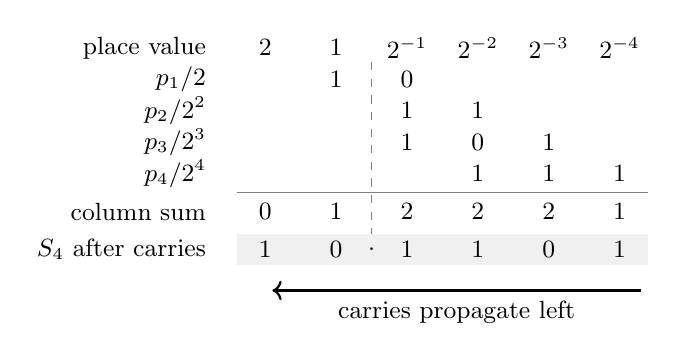
\begin{tikzpicture}[x=0.9cm,y=0.40cm,font=\small]
 \node[anchor=east] at (-0.7,0) {place value};
 \foreach \x/\v in {0/2,1/1,2/{2^{-1}},3/{2^{-2}},4/{2^{-3}},5/{2^{-4}}}
   {\node at (\x,0) {$\v$};}
 \draw[gray,dashed] (1.5,-0.45)--(1.5,-6.9);
 \node[anchor=east] at (-0.7,-1) {$p_1/2$};
 \node at (1,-1) {$1$}; \node at (2,-1) {$0$};
 \node[anchor=east] at (-0.7,-2) {$p_2/2^2$};
 \node at (2,-2) {$1$}; \node at (3,-2) {$1$};
 \node[anchor=east] at (-0.7,-3) {$p_3/2^3$};
 \node at (2,-3) {$1$}; \node at (3,-3) {$0$}; \node at (4,-3) {$1$};
 \node[anchor=east] at (-0.7,-4) {$p_4/2^4$};
 \node at (3,-4) {$1$}; \node at (4,-4) {$1$}; \node at (5,-4) {$1$};
 \draw[gray] (-0.4,-4.6)--(5.4,-4.6);
 \node[anchor=east] at (-0.7,-5.2) {column sum};
 \foreach \x/\v in {0/0,1/1,2/2,3/2,4/2,5/1}
   {\node at (\x,-5.2) {$\v$};}
 \fill[gray!12] (-0.4,-6.9) rectangle (5.4,-5.9);
 \node[anchor=east] at (-0.7,-6.4) {$S_4$ after carries};
 \foreach \x/\v in {0/1,1/0,2/1,3/1,4/0,5/1}
   {\node at (\x,-6.4) {$\v$};}
 \node at (1.5,-6.4) {$.$};
 \draw[<-,thick] (0.1,-7.7)--(5.3,-7.7)
   node[midway,below] {carries propagate left};
\end{tikzpicture}
\caption{Binary addition of the first four terms:
$S_4=\sum_{n=1}^4p_n2^{-n}=(10.1101)_2$.
Overlapping blocks produce column sums greater than one, so carries
propagate left. The omitted infinite tail can change earlier digits.}
\label{fig:carries}
\end{figure}

Tao suggested controlling about $\log\log n$ consecutive gaps by a
sufficiently uniform prime-tuples hypothesis \cite{taoforum}.

Nonconstant numerators need not give normal series: for every
integer $B\ge2$, telescoping gives unconditionally
\[
 \sum_{n\ge1}(Bg_n-g_{n+1})B^{-n}=g_1=1.
\]
The one-point test detects exactly these telescopes (Lemma~\ref{lem:onepoint}).
Algebra computes the local boundary relations; the arithmetic theorem
excludes further rational relations in the stated range.

\paragraph{The basic recurrence.}
For the linear gap series,
\[
 U(n)=\sum_{i\ge1}B^{-i}g_{n+i-1},\qquad U(n+1)=BU(n)-g_n.
\]
Modulo one, the index shift multiplies by $B$. Rationality means eventual
periodicity of this orbit; normality means equidistribution.

\subsection{Main results}\label{sec:mainresults}

Throughout, unqualified logarithms are natural, $B\ge2$ is an integer,
and $\e(t)=\exp(2\pi i t)$.
Normality to base $B$ is equivalent to equidistribution of $(B^N\alpha)_{N\ge0}$
modulo one, by testing base-$B$ cylinder intervals. Its Fourier form
is Weyl's criterion \cite{weyl}. For an increasing positive
integer sequence $a_n$ put $g_n=a_{n+1}-a_n$. Given a fixed period $k$,
write $\bar n\in\{1,\ldots,k\}$ for the representative of $n\bmod k$.
For $F=(F_1,\ldots,F_k)$, each $F_r\in\Q[u_0,\ldots,u_w]$, define,
whenever the series converge,
\[
 \alpha_F(a;B)=\sum_{n\ge1}B^{-n}F_{\bar n}(g_n,\ldots,g_{n+w}),
 \qquad
 W_{r,d}(a;B)=\sum_{m\ge0}g_{km+r}^{\,d}B^{-km-r}.
\]
Reindexing exchanges a gap shift for a factor $B$ and cycles the
period label. The cyclic normal form $\mathcal N_{B,k}$ sends constant
tuples to zero.
If a nonconstant monomial lies in component $r$ and its least gap index is
$j$, shift that index to zero, move to component $\overline{r+j}$, and
multiply by $B^j$; extend linearly.
Section~\ref{sec:algebra} proves that this removes precisely the
cyclic weighted telescopes.

The one-sided averaged Hardy--Littlewood hypothesis
\textup{(AHL$_\kappa$)}, stated in \eqref{eq:ahl}, concerns
tuples of size $O_\kappa(\log\log X)$ in windows of length
$O_\kappa(\log X\log\log X)$. It asks only that the weighted sum of
the adverse errors is $o(X/\log X)$. Their direction alternates with
tuple order, including undercounts. No gap law or digital cancellation
is assumed; $\kappa$ fixes the available window depth.
It implies the weaker positive-comparison condition
\eqref{eq:dominationinput} with $c=1$, which suffices for the theorem below.

\begin{theorem}[Periodic local prime-gap series]\label{thm:prime}
Fix $\kappa>0$ and assume \eqref{eq:dominationinput} for the prime profile
of Section~\ref{sec:primeadapter} with this $\kappa$, for some fixed
$c\ge1$. Fix integers $B\ge2$, $D,k\ge1$ with $D/\log B\le\kappa$.
For every fixed rational local polynomial tuple $F$ with
$\deg\mathcal N_{B,k}F\le D$, the actual prime-gap series $\alpha_F$
is rational if $\mathcal N_{B,k}F=0$ and normal to base $B^k$
(and hence to base $B$) otherwise. For any finite family in this range,
\[
 \sum_iq_i\alpha_{F_i}\in\Q
 \quad\Longleftrightarrow\quad
 \sum_iq_i\mathcal N_{B,k}F_i=0\qquad(q_i\in\Q).
\]
Independent normal forms give jointly equidistributed $B^{kN}$-orbits
and rational linear independence with $1$. Families with different
fixed periods are first repeated into the least common multiple of
their periods, where independence is tested.
\end{theorem}

Every separately fixed width, period and Fourier mode uses the same
window parameters.
For $w=0$, the zero class means that every $F_r$ is constant.
Thus the theorem includes all nonconstant periodic single-gap
polynomials and the joint orbit equidistribution of $W_{r,d}$.
Kuperberg's Conjecture~1.3 implies every fixed
\textup{(AHL$_\kappa$)} by Section~\ref{sec:primeadapter}, so all
separately fixed degrees and bases are covered.

\begin{table}[t]
\centering
\begin{tabular}{@{}lll@{}}
\toprule
Numerator $F$ & Normal form $\mathcal N_{B,1}F$ & Series value or property\\
\midrule
$u_0$ & $u_0$ & normal\\
$u_0^2$ & $u_0^2$ & normal\\
$u_0u_1$ & $u_0u_1$ & normal\\
$Bu_0-u_1$ & $0$ & $g_1=1$\\
$u_0+Bu_0^M-u_1^M$ & $u_0$ & $\alpha_{u_0}+1$, normal\\
\bottomrule
\end{tabular}
\caption{Prime-gap examples at period one. Normality requires only
$\deg(\mathcal N_{B,1}F)/\log B\le\kappa$. The last row, for any fixed
$M\ge2$, therefore needs only the degree-one input. The rational
boundary identities are unconditional.}
\label{tab:examples}
\end{table}

\begin{corollary}[Erd\H os problem 251 and periodic position weights]
\label{cor:erdos251}
Under the arithmetic hypothesis of Theorem~\ref{thm:prime},
for every integer $B\ge2$ with
$1/\log B\le\kappa$ and every nonzero rational periodic sequence $c_n$,
the series $\sum_{n\ge1}c_np_nB^{-n}$ is normal to base $B$.
In particular, $\kappa\ge1/\log2$ implies the normality, and hence
irrationality, of $\sum p_n2^{-n}$. Kuperberg's conjecture suffices.
\end{corollary}
Section~\ref{sec:consequences} proves this by finite Abel transformation.
The square-gap series $\sum g_n^2/2^n$ is also covered by
Theorem~\ref{thm:prime} in its degree-two range, unlike $\sum p_n^2/2^n$.
For the linear prime series, Appendix~\ref{app:quantitative} gives the
quantitative bound \eqref{eq:discrepancy} under Kuperberg's conjecture,
using a finite version of the same positive-comparison input.

\begin{theorem}[Unconditional rough-integer series]\label{thm:rough}
There is an absolute finite $A_*$ such that the classification,
rational-relation and joint-orbit conclusions of Theorem~\ref{thm:prime}
hold unconditionally for the gaps of the increasing enumeration of
$\mathcal R_z=\{a:P^-(a)>z(a)\}$ if, for the fixed $B,D$,
\begin{equation}\label{eq:roughrangeintro}
 \begin{gathered}
 z(x)=\exp(\Psi(\log x)),\qquad \Psi\in C^1,\quad \Psi(t)\to\infty,\\
 0\le t\Psi'(t)\le C_\Psi\Psi(t),\qquad
 \frac t{\Psi(t)}\ge A_*\frac D{\log B}\log(3\Psi(t))
                    \quad\text{eventually}.
 \end{gathered}
\end{equation}
The constant is independent of separately fixed widths, coefficients
and periods. Finite initial conventions are harmless.
\end{theorem}

Here $P^-(a)$ denotes the least prime factor for $a>1$, and $P^-(1):=\infty$.

This includes $z(x)=x^{1/(C\log\log x)}$ for sufficiently large
$C=C(B,D)$. If $\Psi(t)\log(3\Psi(t))=o(t)$, the same rough
sequence supports all separately fixed degrees and bases; for example,
$z(x)=x^{1/(\log\log x\,\log\log\log x)}$ eventually. Different bases
give different numbers, not absolute normality of one number.
No fixed exponent $z(x)=x^\delta$, $\delta>0$, is obtained.

\subsection{Overview of the proof}\label{sec:overview}

Proposition~\ref{prop:localconsumer} transfers local pattern and tail
estimates to normality. Primes and rough integers are two instances.
Integrality gives the recurrence; local variation gives regularity;
the arithmetic comparison transports it; invariance identifies Lebesgue measure.
The polynomial algebra decides when the local variation is present.

\emph{Local variation.}
In the sieve model, not the prime sequence, fix all survivors except $x_j$.
The remaining configuration is a complete frame. The adjacent gaps
$v,W-v$ contribute
\[
 B^{-j-1}\bigl(Bv+W-v\bigr)=B^{-j-1}\bigl((B-1)v+W\bigr).
\]
This nonzero slope is the linear source of regularity
(Figure~\ref{fig:resampling}).

\emph{Regularity and invariance.}
Averaging complete frames without a slot normalization, the Selberg
bound in Section~\ref{sec:model} dominates positive phase tests by
interval integrals. The resulting dominating measure is absolutely
continuous, excluding a rational value with its finite orbit.
The recurrence supplies invariance; the classical principle behind
hot-spot criteria (Lemma~\ref{lem:rigidity}) then gives normality.
No prime exponential-sum estimate is used as arithmetic input.

\emph{The exact exceptions.}
Lemma~\ref{lem:onepoint} identifies invisibility with telescoping to a
rational boundary. Otherwise the leading action has an absolutely
continuous interval image on almost every limiting frame.
The first-gap mean keeps the dominating measure finite;
the $k$-step recurrence handles periodic coefficients.

\emph{Arithmetic and scale.}
The normal-form degree $d$ requires rank $j=d\log_B G+O(1)$;
telescoping terms cost no depth.
For primes, $G=\log X$ explains the $\log\log X$ depth and
$D/\log B\le\kappa$; the reserve controls the infinite tail.
Stopped Bonferroni converts the one-sided tuple hypothesis to pattern
comparison; first-gap averages bound the tail
(Section~\ref{sec:primeadapter}). Appendix~\ref{app:rough} supplies
these inputs unconditionally.

\begin{figure}[t]
\centering
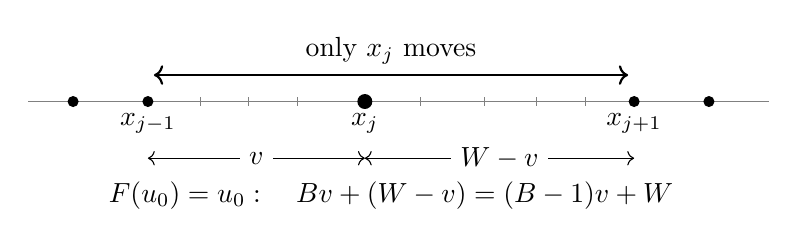
\begin{tikzpicture}[x=0.95cm,y=0.8cm]
 \draw[gray] (-0.6,0)--(9.3,0);
 \foreach \x in {0,1,7.5,8.5}{\fill (\x,0) circle (2pt);}
 \foreach \x in {1.7,2.35,3,3.9,4.65,5.5,6.2,6.85}
   {\draw[gray] (\x,-0.07)--(\x,0.07);}
 \fill (3.9,0) circle (2.7pt);
 \draw[<->,thick] (1.08,0.42)--(7.42,0.42);
 \node[above] at (4.25,0.44) {only $x_j$ moves};
 \node[below] at (1,-0.04) {$x_{j-1}$};
 \node[below] at (3.9,-0.04) {$x_j$};
 \node[below] at (7.5,-0.04) {$x_{j+1}$};
 \draw[<->] (1,-0.9)--node[fill=white] {$v$}(3.9,-0.9);
 \draw[<->] (3.9,-0.9)--node[fill=white] {$W-v$}(7.5,-0.9);
 \node[below] at (4.25,-1.12)
   {$F(u_0)=u_0:\quad Bv+(W-v)=(B-1)v+W$};
\end{tikzpicture}
\caption{One-point variation in the sieve model. Ticks mark eligible
presieve sites between the fixed neighbours. The proof averages
unnormalized insertion sums over all complete frames, including empty
slots (see \eqref{eq:frameaverage}). The linear action has nonzero slope
for $B>1$.}
\label{fig:resampling}
\end{figure}

\subsection{Related work}\label{sec:relatedwork}

Land independently proved conditional irrationality of $\sum p_n2^{-n}$
under Kuperberg's conjecture before the present work appeared \cite{land}.
He selects rare prime patterns and averages to control the tail;
our local averaging yields normality and the polynomial classification.
No implication between the two specialized local hypotheses is claimed.

Gallagher obtains Poisson statistics from uniform fixed-order tuple
estimates \cite{gallagher}; our tests need growing order, as allowed by
Kuperberg's conjecture \cite{kuperberg}. Tao also compares primes with
a random sieve \cite{tao2023}. Banks--Ford--Tao's signed averaged input
\cite{bft} does not automatically control our one-sided error norm.

Copeland--Erd\H os concatenate primes without carries \cite{copelanderdoes};
Nakai--Shiokawa extend this to positive integer-valued nonconstant
polynomials evaluated at primes \cite{nakaishiokawa}, and Madritsch
treats rounded pseudo-polynomials, including nonintegral powers
\cite{madritsch2014}. These are concatenations, whereas our gap series
have overlapping contributions and carries.
Bailey--Crandall and Lagarias connect arithmetical series with digit
orbits \cite{baileycrandall,lagarias}; we instead establish regularity
by positive comparison, without verifying their Hypothesis~A.
Bailey--Crandall also construct uncountable normal families
\cite[Theorem~4.12]{baileycrandall}. Corollary~\ref{cor:roundedpowers}
provides a concrete gap-parametrized family with rational linear
independence and joint orbit equidistribution of every fixed finite subfamily.

Kova\v{c}'s variable-denominator counterexample chooses integers $q_n\ge2$,
$q_n=o(p_n)$, without requiring monotonicity, so that
$\sum p_n/(q_1\cdots q_n)$ telescopes \cite{kovacforum}.
Our geometric weights, in contrast, are fixed in advance.

Pratt proved irrationality of $\sum\omega(n)2^{-n}$ conditionally on
uniform prime tuples \cite{pratt}; Tao--Ter\"av\"ainen proved it
unconditionally \cite{taoteravainen}. Here $\omega(n)$ counts distinct
prime factors. Their multiplicative correlation input does not supply
our rank-dependent prime-pattern comparison.
Figure~\ref{fig:confluence} summarizes the connections behind the proof.

\section[Telescopes and the one-point test]{Cyclic telescopes and the one-point test}\label{sec:algebra}

Let $\mathcal G=\Q[u_0,u_1,\ldots]$ with finite variable support and
$\mathsf S u_i=u_{i+1}$. The combined shift on $\mathcal G^k$ is
$(\mathsf AH)_r=\mathsf S H_{\overline{r+1}}$, and
\[
 \mathcal T_B=B-\mathsf A,\qquad
 (\mathcal T_BH)_r=BH_r-\mathsf S H_{\overline{r+1}}.
\]
For example, at period $k=2$, $\mathsf A(u_0,0)=(0,u_1)$.
The local cohomological equation $(B-\mathsf A)H=F$ asks for a
polynomial primitive with finite variable support. The same geometric
reindexing gives the finite boundary formula \eqref{eq:localboundary}
and the $k$-step recurrence \eqref{eq:sharedrecursion}.
The normal form below computes the obstruction to local solvability;
the converse from rationality of the series will require arithmetic.

Write $e_rM$ for the tuple with $M$ in component $r$ and zero elsewhere.
For a nonconstant monomial $M=\mathsf S^jM^\flat$ with $u_0\mid M^\flat$,
define
\[
 \mathcal N_{B,k}(e_rM)=B^j e_{\overline{r+j}}M^\flat,
 \qquad \mathcal N_{B,k}(\text{constant tuple})=0.
\]
Degree of a tuple means the maximum component degree, with $\deg0=-\infty$.

\begin{lemma}[Cyclic normal form]\label{lem:localnormalform}
Every $F\in\mathcal G^k$ has a unique decomposition
$F=\mathcal N_{B,k}F+\mathcal T_BH$.
It preserves degree bounds and
$\ker\mathcal N_{B,k}=\mathcal T_B\mathcal G^k$.
\end{lemma}
\begin{proof}
Every nonconstant labelled monomial belongs to exactly one chain
$\mathsf A^jC$ ($j\ge0$), starting at $C=e_qM^\flat$ with
$u_0\mid M^\flat$: indeed
$\mathsf A^jC=e_{\overline{q-j}}\mathsf S^jM^\flat$.
Thus uniquely $F=c+\sum_C p_C(\mathsf A)C$, with a constant tuple $c$.
Ordinary polynomial division gives
\[
 p_C(z)=p_C(B)+(B-z)q_C(z),\qquad
 \mathcal N_{B,k}F=\sum_Cp_C(B)C.
\]
The primitive is $\sum_Cq_C(\mathsf A)C+H_c$, where
\[
 H_c=(B^k-1)^{-1}\sum_{i=0}^{k-1}B^{k-1-i}\mathsf A^ic.
\]
Here $\mathsf A^kc=c$. Division on each chain and this inverse on
constants prove uniqueness. Gap degree is constant along a chain,
so both operations preserve degree bounds. If $F$ uses only indices
at most $w$, every nonconstant term of $H$ uses indices at most $w-1$.
Moreover,
$\mathcal N_{B,k}\mathsf A=B\mathcal N_{B,k}$ and the kernel is
$\mathcal T_B\mathcal G^k$.
\end{proof}
Since $\mathcal N_{B,k}$ cannot increase degree and is unchanged by
subtracting $\mathcal T_BH$, the canonical decomposition attains the
least degree in each nonzero class modulo telescopes.

Evaluation gives the finite identity
\begin{equation}\label{eq:localboundary}
 \alpha_F^{[N]}-\alpha_{\mathcal N_{B,k}F}^{[N]}
 =H_{\bar1}(g_1,\ldots)-B^{-N}H_{\overline{N+1}}(g_{N+1},\ldots),
\end{equation}
where superscript $[N]$ denotes truncation at $n=N$.
Whenever the endpoint vanishes, the series difference is rational;
Lemma~\ref{lem:derivedgrowth} ensures this under (S).
Thus the series modulo $\Q$ depends only on the vector-space class
of $F$ modulo $\mathcal T_B\mathcal G^k$.
Within the effective-degree range, the arithmetic theorem rules out
further rational relations and proves normality for every nonzero class.
Without arithmetic the converse fails: $a_n=n^2$ gives
$\alpha_{u_0}=(3B-1)/(B-1)^2\in\Q$ although
$\mathcal N_{B,1}u_0=u_0$.

In the action below, shifts also act on integer-indexed gap variables.
\begin{lemma}[Telescopes and local invisibility]\label{lem:onepoint}
For $F\in\mathcal G^k$ using $u_0,\ldots,u_w$, set
$u_{-1}=v$, $u_0=W-v$ and define
\begin{equation}\label{eq:localaction}
 \pi_s(v;y)=\sum_{t=-w-1}^{0}B^{-t}
       F_{\overline{s+t+1}}(u_t,\ldots,u_{t+w}),
\end{equation}
where $y$ consists of $W$ and the exterior gaps. Then
\[
 \mathcal N_{B,k}F=0
 \ \Longleftrightarrow\ F=\mathcal T_BH\text{ for some }H
 \ \Longleftrightarrow\ \partial_v\pi_s\equiv0\text{ for every }s,
\]
as polynomial identities in $v,y$.
Moreover, if $F=\mathcal N_{B,k}F\ne0$ has degree $d$, some
action has a degree-$d$ homogeneous part nonconstant in $v$.
\end{lemma}
\begin{proof}
First let $F=\mathcal N_{B,k}F\ne0$ have degree $d$, and let
$P=F^{[d]}$ be its top homogeneous part. The normal form acts degree
by degree, so $P$ is again normal. Write $\pi_s(P)$ for its action:
the linear substitution makes this exactly the degree-$d$ part of
$\pi_s(F)$. Let $h$ be the greatest variable index of $P$.
If $h\ge1$, choose a component $r$ with $\partial_{u_h}P_r\ne0$
and put $s=\overline{r+h}$.
Before substituting $u_{-1}=v$, $u_0=W-v$, the derivative
$(\partial_{u_{-1}}-\partial_{u_0})\pi_s(P)$ has just one term
depending on $u_{-h-1}$:
\[
 B^{h+1}\mathsf S^{-h-1}\partial_{u_h}P_r.
\]
It really depends on that variable, since every normal monomial
contains $u_0$. Earlier summands $t<-h-1$ use only $u_t,\ldots,u_{t+h}$,
so neither moved gap occurs and their derivatives vanish.
Thus the derivative is nonzero,
also after the invertible substitution. If $h=0$, all derivatives
could vanish only if $BP_s'(u_{-1})=P_{\overline{s+1}}'(u_0)$
for every $s$. The independent variables force constant derivatives
$a_s$ with $Ba_s=a_{\overline{s+1}}$; hence $(B^k-1)a_s=0$,
contradicting $P\ne0$.

For general $F$, use the normal-form decomposition. A telescope
$F=\mathcal T_BH$ contributes only the exterior boundary
\[
 \pi_s(F)=B^{w+2}(\mathsf S^{-w-1}H)_{\overline{s-w}}
                     -(\mathsf SH)_{\overline{s+2}};
\]
if $H$ is not constant its largest index is at most $w-1$.
The normal-part argument and Lemma~\ref{lem:localnormalform}
prove both equivalences.
\end{proof}
This is a weighted polynomial instance of the discrete variational
principle that a density invisible to all interior variations is a
boundary term; compare \cite{hydonmansfield}. The direct proof above
requires none of the general variational machinery.

\section{A common digital criterion}\label{sec:criterion}

\subsection{Pattern assumptions and rigidity}\label{sec:patternrigidity}

Let $a_n$ increase through positive integers and fix a real auxiliary
scale $\rho>1$, not necessarily an integer digit base; write
$\kappa=1/\log\rho$. For every sufficiently
large integer $X$ set
\begin{equation}\label{eq:profile}
 \begin{gathered}
 G_X\to\infty,\qquad L=L_X=\left\lceil\log_\rho G_X+\sqrt{\log_\rho G_X}\right\rceil,
 \qquad S=S_X=\lfloor(6/5)LG_X\rfloor,\\
 I_X=\{n:X<a_n\le2X\},\qquad m_X=|I_X|>0,\qquad
 T_\rho(n)=\sum_{h\ge1}g_{n+h-1}\rho^{-h}.
 \end{gathered}
\end{equation}
Here $n$ is a sequence index and $X$ a value bound;
$L$ counts gaps, whereas $S$ is a physical span.
For a nonempty finite index set $I$, write
$\Avg_{n\in I}f(n)=|I|^{-1}\sum_{n\in I}f(n)$.
Write $V(y)=\prod_{p\le y}(1-1/p)$. The rooted sieve law $\Prob_{0,y}$
excludes one independent uniform nonzero residue at each prime $p\le y$;
write its nonnegative survivors as $0=x_0<x_1<\cdots$.
Thus the origin, or root, is always retained.

(S) compares initial patterns with a calibrated sieve; (T) bounds the
tail in mean. Neither assumption mentions digits.
There are probability mixtures
$\omega_X$ of these laws with
$\sup_{y\in\operatorname{supp}\omega_X}|V(y)^{-1}/G_X-1|\to0$ such that,
uniformly over complex first-$L$ tests $f$ with $|f|\le1$ and
$f=0$ when $x_L>S$,
\begin{align}
 \Avg_{n\in I_X}f(a_{n+1}-a_n,\ldots,a_{n+L}-a_n)
   &=\int\E_{0,y}f(x_1,\ldots,x_L)\,d\omega_X(y)+o(1),\tag{S}\label{eq:S}\\
 \Avg_{n\in I_X}T_\rho(n+L)&=O_\rho(G_X).\tag{T}\label{eq:T}
\end{align}
The test may depend on $X$. The infinite remainder (T) is about the
actual sequence, not an infinite model observable. Its series is
well-defined by the following consequence of (S); the quantitative mean
bound in (T) remains a separate assumption. The model estimates used
here are proved in Section~\ref{sec:model}.

\begin{lemma}[Growth from local pattern comparison]\label{lem:derivedgrowth}
Condition (S) implies $m_X\to\infty$ and $\log a_n/n\to0$.
Consequently every fixed local polynomial series with geometric
denominator converges absolutely, and all boundaries in
\eqref{eq:localboundary} vanish.
\end{lemma}
\begin{proof}
(S) and the model span bound make the actual mass on $x_L\le S$
tend to one. A fixed location $1\le d\le S$ survives the independent
prime coordinates $S<p\le y$ with probability
\[
 \prod_{S<p\le y}(1-1/(p-1))
       \le V(y)/V(S)\ll\log S/G_X=o(1),
\]
uniformly in calibrated mixtures. Choose $n\in I_X$ with
$a_{n+L}-a_n\le S$, and put $d_X=g_n$.
(S) on $\ind_{\{x_1=d_X,\,x_L\le S\}}$
gives $1/m_X\le\epsilon_X+O(\log S/G_X)\to0$, where
$\epsilon_X\to0$ is the uniform error in (S). Thus $m_X\to\infty$,
without using a spacing limit.

Fix $K$. For all sufficiently large integers $J$,
$A(2^J)\ge K(J-J_0)$, by summing over disjoint dyadic intervals in the values of the sequence;
here $A(x)=\#\{n:a_n\le x\}$.
If $2^J\le a_n<2^{J+1}$, then
$\log a_n\le(n/K+J_0+1)\log2$.
Let $n\to\infty$, then $K\to\infty$.
Every fixed shifted polynomial value has absolute value at most $\exp(o(n))$,
which proves the last assertions. No mean-tail estimate follows from
this growth argument alone.
\end{proof}

Write $\lambda$ for normalized Lebesgue measure on
$\mathbb T=\R/\Z$ and $T_Cx=Cx\bmod1$.
The following classical principle also underlies hot-spot criteria
\cite[Lemma 3.2]{baileymisiurewicz}.

\begin{lemma}[Absolute continuity, invariance and rational lifts]
\label{lem:rigidity}
For an integer $C\ge2$, a $T_C$-invariant probability
$\mu\ll\lambda$ equals $\lambda$.
If $q\alpha$ is normal to base $C$ for an integer $q\ge1$, then
$\alpha$ is normal to base $C$. Consequently rational affine maps
with nonzero slope preserve normality.
\end{lemma}
\begin{proof}
For $t\in\Z\setminus\{0\}$, invariance and Riemann--Lebesgue give
$\widehat\mu(t)=\widehat\mu(C^ht)\to0$, so $\mu=\lambda$.
If $q\alpha$ is normal, any empirical limit $\nu$ of the
$C$-orbit of $\alpha$ is invariant and $(T_q)_*\nu=\lambda$.
For compact $\lambda$-null $K$, its image $T_qK$ is compact and null,
and
\[
 \nu(K)\le\nu(T_q^{-1}(T_qK))=\lambda(T_qK)=0.
\]
Inner regularity gives $\nu\ll\lambda$, hence $\nu=\lambda$.
Integer multiples preserve normality by Weyl's criterion.
For a rational affine map, clear denominators and use this lift.
\end{proof}
The last assertion is Wall's normality-preservation theorem
\cite{wall}; see also \cite[Proposition 4.25 and Remark 4.28]{bergelsondownarowicz}.
Lyons constructed a measure with vanishing Fourier coefficients
carried by numbers not normal to base $2$ \cite{lyons1986}.
Here the additional invariance identifies the limiting measure itself
with Lebesgue measure.

\subsection{The digital transfer criterion}\label{sec:commonproof}

\begin{proposition}[Digital transfer criterion]\label{prop:localconsumer}
Assume (S)/(T). Fix integers $B\ge2$, $D,k\ge1$ with $B\ge\rho^D$.
For any rational local tuple $F\in\mathcal G^k$ with
$\deg\mathcal N_{B,k}F\le D$, its series $\alpha_F$
is rational if $\mathcal N_{B,k}F=0$, and normal to base $B^k$
(and hence to base $B$) otherwise.
\end{proposition}
\begin{proof}
Lemma~\ref{lem:derivedgrowth} justifies all polynomial series and
boundaries. Apply Lemma~\ref{lem:localnormalform},
\eqref{eq:localboundary} and the rational-affine lift
in Lemma~\ref{lem:rigidity}; it suffices to treat an integral normal tuple
$F=\mathcal N_{B,k}F\ne0$ of degree $d\le D$ and fixed width $w+1$.

\smallskip\noindent\emph{Step 1. Recurrence and truncation.}
Set
\[
 U(n)=\sum_{i\ge1}B^{-i}
          F_{\bar i}(g_{n+i-1},\ldots,g_{n+i+w-1}).
\]
Then $U(1)=\alpha_F$, and exact reindexing gives
\begin{equation}\label{eq:sharedrecursion}
 U(n+k)=B^kU(n)-\sum_{i=1}^k B^{k-i}
                   F_{\bar i}(g_{n+i-1},\ldots,g_{n+i+w-1}),
\end{equation}
where the subtracted sum is an integer. The labels are relative to $i$, not $n$.

For the window length $L=L_X$, put $K=L-w$ and write the truncation as
a function of the first $L$ offsets, with $h_i=x_{i+1}-x_i$:
\[
 \Phi_K(x)=\sum_{i=1}^{K}B^{-i}
                    F_{\bar i}(h_{i-1},\ldots,h_{i+w-1}).
\]
At the actual root $n$ substitute $x_i=a_{n+i}-a_n$ and write
$\Phi_K(n)$.

Write $G=G_X$. For positive integer gaps, $|F_r(z)|^{1/d}\ll_F\sum_jz_j$.
Subadditivity, $B^{-i/d}\le\rho^{-i}$ and reindexing give
\[
 |U(n)-\Phi_K(n)|^{1/d}
       \le c_{F,\rho}\rho^{-K}T_\rho(n+K).
\]
Put $\psi(t)=\min(1,t)$. Shifting the bounded sequence
$\psi(c_{F,\rho}\rho^{-K}T_\rho(n+K))$ by $w=L-K$ costs at most
$2w/m_X$, so (T) and $\rho^{-K}=\rho^w\rho^{-L}$ give
\[
 \Avg_{n\in I_X}\psi\bigl(|U(n)-\Phi_K(n)|^{1/d}\bigr)
 \le c_{F,\rho}\rho^{-K}\Avg_{n\in I_X}T_\rho(n+L)
                         +\frac{2w}{m_X}\longrightarrow0.
\]
Here $G\rho^{-L}\le\rho^{-\sqrt{\log_\rho G}}\to0$.
Uniform continuity transfers every fixed continuous phase test.
Condition (S) bounds the mass omitted by the span restriction.

\smallskip\noindent\emph{Step 2. One-point variation at the critical rank.}
Moving a point $x_j$, with
$w+1\le j\le K-1$, changes the phase by its variable part
$B^{-j-1}\pi_s(v;y)$, where $s\equiv j\pmod k$,
$v=x_j-x_{j-1}$, and $y$ consists of
$W=x_{j+1}-x_{j-1}$ and the interacting exterior gaps.

Apply Lemma~\ref{lem:onepoint} to the normal tuple.
For some residue $s$, the degree-$d$ homogeneous
part of $\pi_s$ is nonconstant in $v$. This single check covers all
periods and all fixed local widths.

Put $C=B^k$. Choose once $j_X\equiv s\pmod k$ with
\[
                  \theta_X=G^dB^{-j_X-1}\in[1,C).
\]
The degree/base inequality and the reserve give
$w+1\le j_X\le L-w-1$ eventually.
This rank is independent of the Fourier mode and accuracy
(Figure~\ref{fig:scale}).

\begin{figure}[t]
\centering
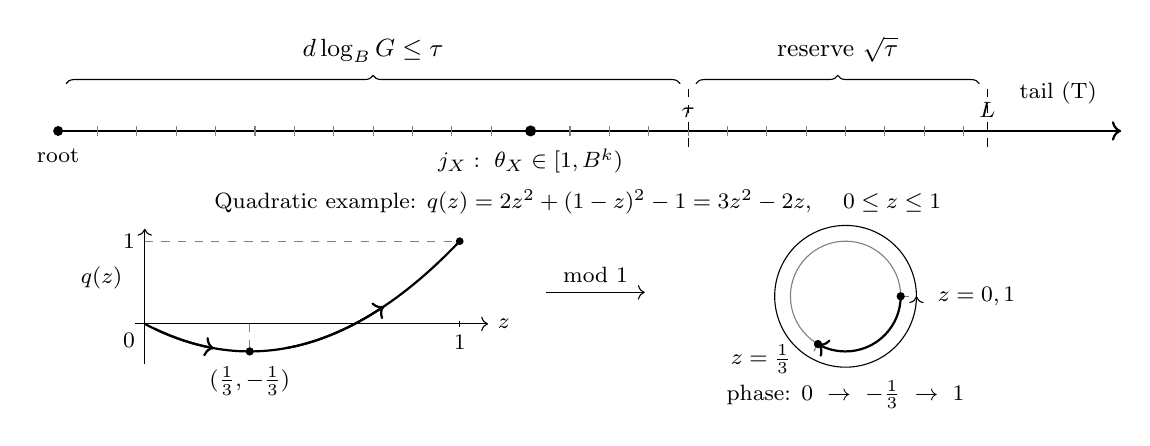
\begin{tikzpicture}[font=\small,x=1cm,y=1cm]
 \draw[->,thick] (0,0)--(13.5,0);
 \foreach \x in {0,0.5,...,11.5}{\draw[gray] (\x,-0.06)--(\x,0.06);}
 \fill (0,0) circle (1.8pt);
 \node[below,font=\footnotesize] at (0,-0.1) {root};
 \fill (6,0) circle (2pt);
 \node[below,font=\footnotesize] at (6,-0.1) {$j_X:\ \theta_X\in[1,B^k)$};
 \draw[dashed] (8,-0.2)--(8,0.55);
 \draw[dashed] (11.8,-0.2)--(11.8,0.55);
 \node[above,font=\footnotesize] at (8,0.05) {$\tau$};
 \node[above,font=\footnotesize] at (11.8,0.05) {$L$};
 \draw[decorate,decoration={brace,amplitude=3pt}]
   (0.1,0.6)--(7.9,0.6) node[midway,above=4pt] {$d\log_B G\le\tau$};
 \draw[decorate,decoration={brace,amplitude=3pt}]
   (8.1,0.6)--(11.7,0.6) node[midway,above=4pt] {reserve $\sqrt\tau$};
 \node[font=\footnotesize] at (12.7,0.48) {tail (T)};

 \node[font=\footnotesize] at (6.6,-0.9)
   {Quadratic example: $q(z)=2z^2+(1-z)^2-1=3z^2-2z$, \quad $0\le z\le1$};
 \begin{scope}[shift={(1.1,-2.45)},x=4cm,y=1.05cm]
  \draw[->] (0,-0.48)--(0,1.15);
  \node[left,font=\footnotesize] at (-0.04,0.55) {$q(z)$};
  \draw[->] (-0.03,0)--(1.09,0) node[right,font=\footnotesize] {$z$};
  \draw[gray,dashed] (0,1)--(1,1);
  \draw[gray,dashed] (0.333333,0)--(0.333333,-0.333333);
  \node[left,font=\footnotesize] at (0,1) {$1$};
  \node[below left,font=\footnotesize] at (0,0) {$0$};
  \draw (1,-0.035)--(1,0.035);
  \node[below,font=\footnotesize] at (1,-0.02) {$1$};
  \draw[thick,domain=0:1,samples=81] plot (\x,{3*\x*\x-2*\x});
  \draw[->,thick,domain=0.03:0.22,samples=15] plot (\x,{3*\x*\x-2*\x});
  \draw[->,thick,domain=0.45:0.76,samples=20] plot (\x,{3*\x*\x-2*\x});
  \fill (0.333333,-0.333333) circle (1.5pt);
  \fill (1,1) circle (1.4pt);
  \node[below,font=\footnotesize] at (0.333333,-0.40) {$(\tfrac13,-\tfrac13)$};
 \end{scope}
 \draw[->] (6.2,-2.05)--(7.45,-2.05)
   node[midway,above,font=\footnotesize] {mod $1$};

 % Same phase circle; the return trace is displaced radially for legibility.
 \draw[gray] (10.0,-2.1) circle (0.70);
 \draw[thick,->] (10.70,-2.1)
   arc[start angle=0,end angle=-120,radius=0.70];
 \draw[gray,dashed] (9.65,-2.706218)--(9.55,-2.879423);
 \draw[->] (9.55,-2.879423)
   arc[start angle=-120,end angle=360,radius=0.90];
 \draw[gray,dashed] (10.70,-2.1)--(10.90,-2.1);
 \fill (10.70,-2.1) circle (1.5pt);
 \fill (9.65,-2.706218) circle (1.5pt);
 \node[right,font=\footnotesize] at (11.05,-2.1) {$z=0,1$};
 \node[left,font=\footnotesize] at (9.43,-2.90) {$z=\tfrac13$};
 \node[font=\footnotesize] at (10,-3.35) {phase: $0\ \to\ -\tfrac13\ \to\ 1$};
\end{tikzpicture}
\caption{Scale selection and a quadratic local action.
Above, $\tau=\log_\rho G$ and $L=\lceil\tau+\sqrt\tau\rceil$;
the reserve accommodates fixed width and period and ensures $G\rho^{-L}\to0$.
Below, $F(u_0)=u_0^2$, $B=2$, unit normalized insertion span and
$\theta_X=1$ give $q$ up to an additive constant.
The phase reverses at $z=1/3$; directed traces on the circle are offset
for visibility. The image of uniform length is absolutely continuous,
but not uniform: invariance is still needed.}
\label{fig:scale}
\end{figure}

In the model, let $\mathcal A$ be the sites in $[1,S]$ surviving primes
up to $S$, and $N$ the final survivor count. The auxiliary law $\E^-$
retains the original $(y,\mathcal A,N)$-marginal, restricts to $N\ge L$,
and chooses a uniform $(N-1)$-subset $U^-$ of $\mathcal A$, without
normalizing the restricted mass. It differs from fixed-rank deletion;
\eqref{eq:frameaverage} accounts for the change of law.
The auxiliary local frame $Y_X^-$ consists of the gaps of $U^-$ at
ranks $j_X-w-1,\ldots,j_X+w-1$, divided by $G$.
These ranks lie in $0,\ldots,L-2$, so
Lemma~\ref{lem:localspacings} gives tightness and absolutely continuous
limits. Write $W(Y)$ for its central gap (the insertion span) and
$Q_Y(z)$ for the top homogeneous action in $z=v/G$.
Write $\Phi_K(\mathcal F,u)$ for evaluation after ordered insertion
of $u$ at rank $j_X$; retain repeated entries at slot endpoints.
Define the outer phase on every frame, even one with no eligible
insertion, by polynomial evaluation at its left endpoint $a_{\mathcal F}$:
\[
 O_{\mathcal F}=\Phi_K(\mathcal F,a_{\mathcal F})
              -B^{-j_X-1}\pi_s(0;y_{\mathcal F})\pmod1.
\]
This permits the virtual zero gap. On compact frames, uniformly for
$z=(u-a_{\mathcal F})/G\in[0,W(Y)]$,
\[
 \Phi_K(\mathcal F,u)=O_{\mathcal F}+\theta_XQ_Y(z)+o(1)\pmod1.
\]
The outer phase may vary arbitrarily between
frames, but is independent of the inserted point on each frame.

\smallskip\noindent\emph{Step 3. Positive domination and absolute continuity.}
Put $J_X=\{n\in I_X:n\equiv1\pmod k\}$ and
$\ell_X=|J_X|=m_X/k+O(1)\to\infty$.
Consider any weak limit $\nu$ of the class measures
\[
                  \nu_X=\ell_X^{-1}\sum_{n\in J_X}\delta_{U(n)\bmod1}.
\]
Along a further subsequence the joint auxiliary law of
$(O_{\mathcal F},Y_X^-,\theta_X)$ converges to a probability $\Lambda$:
the circle and $[1,C]$ are compact, and the frame laws are tight.
Place the vanishing missing mass at a fixed point.
This extraction precedes all tests and cutoffs.
The one-point lemma gives a nonzero polynomial in $Y$ among the
coefficients of $\partial_zQ_Y$. Its zero set is Lebesgue-null, so the
absolutely continuous $Y$-marginal makes $Q_Y$ nonconstant
$\Lambda$-almost surely. Since $W\ge0$ is continuous, the gap means
and Portmanteau give $\int W(Y)\,d\Lambda\le2$.

Define a finite measure $\sigma$ on $\mathbb T$ by
\[
 \sigma(f)=\int\!\int_0^{W(Y)}
                 f(O+tQ_Y(z))\,dz\,d\Lambda(O,Y,t).
\]
Then $\sigma(\mathbb T)\le2$ and $\sigma\ll\lambda$.
A nonconstant polynomial has finitely many critical points;
change of variables on its monotone pieces proves absolute continuity
of its interval image. Translation and reduction modulo one preserve it.

Fix $f\ge0$ continuous on $\mathbb T$. Positivity gives
$\nu_X(f)\le(k+o(1))\Avg_{n\in I_X}f(U(n))$.
Choose a continuous compactly supported $0\le\chi_A\le1$ equal to one
on $[0,A]^{2w+1}$. In an original model configuration, delete $x_{j_X}$
and denote the resulting local frame coordinates, divided by $G$, by $Y^{\rm del}$.
The central gap is a sum of two original gaps; the others are single gaps.
The original rooted means therefore give
\[
 \E\!\left[\ind_{\{N\ge L\}}\sum_iY_i^{\rm del}\right]
                          \le(2w+2)(1+o(1)).
\]
Markov bounds the discarded original frame mass by $O_w(A^{-1})$.
Since $Y^{\rm del}(\mathcal F\cup\{u\})=Y(\mathcal F)$ for every admissible
insertion, the same cutoff becomes
$\chi_A(Y_X^-)$ under the auxiliary law. Thus
\[
 \nu_X(f)\le
 24k\,\E^-\!\left[\chi_A(Y_X^-)
       \int_0^{W(Y_X^-)}
          f(O_{\mathcal F}+\theta_XQ_{Y_X^-}(z))\,dz\right]
       +O_{F,k}(A^{-1})\|f\|_\infty+o(1).
\]
Here (S), the span estimate and the remainder bound first transfer the
test on actual offsets to the model. The probabilities of exceptional
counts and large original frames are bounded before changing measure. On the compact cutoff the tests are
equicontinuous, uniformly over the outer phase.
Equations~\eqref{eq:frameaverage} and \eqref{eq:positiveinsertion}
give $12\vartheta G/\log G<24$; positivity permits extension to all
auxiliary frames. The cutoff integral is bounded and jointly continuous
in $(O,Y,t)$. Pass to the fixed joint limit, use $\chi_A\le1$, and then
send $A\to\infty$. This gives $\nu\le24k\sigma$, hence $\nu\ll\lambda$.

\smallskip\noindent\emph{Step 4. Invariance and the full orbit.}
For every continuous $f$, \eqref{eq:sharedrecursion} gives
\[
 |\nu_X(f(C\,\cdot))-\nu_X(f)|
                    \le2\|f\|_\infty/\ell_X\longrightarrow0.
\]
Thus $\nu$ is $T_C$-invariant. Lemma~\ref{lem:rigidity} gives
$\nu=\lambda$, and consequently $\nu_X\Rightarrow\lambda$.

Fix $q\in\Z\setminus\{0\}$ and $\epsilon>0$, and choose $X_0$ so that
every integer $X\ge X_0$ has
$|\Avg_{n\in J_X}\e(qU(n))|\le\epsilon$.
Starting at $b=a_{1+k(N-1)}$, repeatedly take $X=\lfloor b/2\rfloor$,
remove the terms with values in $(X,2X]$, and replace $b$ by $X$;
stop when $b<2X_0$.
Each step omits at most one integer. Lemma~\ref{lem:derivedgrowth}
bounds the number of steps by $O(\log a_{1+k(N-1)})=o(N)$.
The complete blocks contribute at most $\epsilon N$, and the final
bounded interval contributes $O_{X_0}(1)$. Hence
\[
 \frac1N\sum_{h=0}^{N-1}\e(qU(1+kh))\longrightarrow0.
\]
By \eqref{eq:sharedrecursion}, these are the character means of the
$C$-orbit of $\alpha_F$. Weyl's criterion proves normality to $C=B^k$.
For $0\le r<k$, multiplication by $B^r$ preserves Lebesgue measure,
so $(B^{kh+r}\alpha_F)_h$ is equidistributed. Interleaving these
$k$ subsequences gives base-$B$ normality.
\end{proof}

\paragraph{Positive comparison suffices.}
The criterion and its consequences also hold if (S) is replaced by
its upper inequality for $0\le f\le1$, with the model term multiplied
by a fixed $c\ge1$, provided the actual mass outside $x_L\le S$ is $o(1)$.
Keep the same support, uniformity and calibrated mixtures, and (T).
The positive point test still proves Lemma~\ref{lem:derivedgrowth};
Step~3 gives $\nu\le24kc\sigma$. All other steps are unchanged.

\subsection[Relations and positions]{Relations, dimension and positions}\label{sec:consequences}

The rational boundary in \eqref{eq:localboundary} and the criterion
give exactly the rational relations between the normal classes.
Under (S)/(T), fix integers $B\ge2$, $k,H,D\ge1$ with $B\ge\rho^D$.
For period $k$, $H$ gap variables and total degree at most $D$,
the normal monomials are the $k$ labelled copies of
$u_0^{\beta_0}\cdots u_{H-1}^{\beta_{H-1}}$ with $\beta_0\ge1$
and $\sum\beta_i\le D$. Removing one factor $u_0$ gives
\[
 \dim_\Q\operatorname{span}_\Q
 \{1,\alpha_F:F_r\in\Q[u_0,\ldots,u_{H-1}],\ \deg F_r\le D\}
      =1+k\binom{H+D-1}{D-1}.
\]
Every nonzero integer combination of independent normal classes is
normal to $B^k$; scalar Weyl proves the joint orbit assertion.
At $H=1$ these classes are precisely the $kD$ components $W_{r,d}$.

For different fixed periods $k_i$, put $k^*=\operatorname{lcm}(k_i)$
and repeat each tuple into its $k^*$ components. This embedding commutes with
$\mathsf A$ and the normal form: it maps normal
tuples to normal tuples and telescopes to telescopes. It changes no
series value. Test independence after this embedding and apply the
same argument at period $k^*$ along the powers $B^{k^*N}$.

Regard the rational periodic position weights $c_n$ as a constant
$k$-tuple. Using the inverse already computed in
Lemma~\ref{lem:localnormalform}, set
$d=(B-\mathsf A)^{-1}\mathsf Ac$, with periodic indices.
On this constant space $\mathsf A^k=1$, and both factors are
invertible. Thus $c\mapsto d$ is invertible and
$Bd_j-d_{j+1}=c_{j+1}$. Finite telescoping gives
\[
 \sum_{n=1}^N c_na_nB^{-n}
 =a_1d_0+\sum_{j=1}^{N-1}d_jg_jB^{-j}-a_Nd_NB^{-N}.
\]
The endpoint vanishes by Lemma~\ref{lem:derivedgrowth}. Thus nonzero
periodic position weightings are normal, and their residue components
inherit common-$B^k$ joint equidistribution by the scalar character
test and rational-affine invariance. Equation~\eqref{eq:abelbasic} is the
period-one case; no new position-tail estimate is needed.

\subsection{Rounded real gap powers}\label{sec:roundedpowers}

\begin{corollary}[Rounded real gap powers]\label{cor:roundedpowers}
Assume (S)/(T), or the positive-comparison variant of
Proposition~\ref{prop:localconsumer}. Fix integers $B\ge2$, $k\ge1$
with $B\ge\rho$. For $1\le r\le k$ and real $0<\alpha\le1$, put
\[
 V_{r,\alpha}=\sum_{h\ge0}
       \lfloor g_{kh+r}^{\alpha}\rfloor B^{-kh-r}.
\]
Here $\alpha$ denotes an exponent, distinct from the series notation $\alpha_F$.
Every nontrivial finite rational linear combination of this indexed
family is normal to base $B^k$. Every fixed finite subfamily has jointly
equidistributed $B^{kN}$-orbits, and $1$ together with the entire
family is rationally linearly independent.
The same assertions hold with all floors replaced by ceilings.
Moreover, for a nonconstant $P\in\Q[T]$ of degree $m$ and fixed
$0<\alpha\le1/m$, both
$\sum_{n\ge1}P(\lfloor g_n^\alpha\rfloor)B^{-n}$ and its ceiling analogue
are normal to base $B$.
\end{corollary}

\begin{proof}
Clear denominators and group equal exponents, writing
$F_r(q)=\sum_\ell b_{r\ell}\lfloor q^{\alpha_\ell}\rfloor$
with integer coefficients. Let $a>0$ be the largest exponent with a
nonzero coefficient column $(b_r)$. Lemma~\ref{lem:derivedgrowth}
and $|F_r(q)|\ll q$ for integers $q\ge1$ give convergence.
Define $U,\Phi_L$ by the sums in Step~1 of
Proposition~\ref{prop:localconsumer}, with width zero, and put $G=G_X$.
The recurrence \eqref{eq:sharedrecursion} is exact with an integer
subtracted sum, and
\[
 |U(n)-\Phi_L(n)|\ll\rho^{-L}T_\rho(n+L).
\]
Thus (T) and $G\rho^{-L}\to0$ transfer continuous phase tests
using only the degree-one remainder estimate.

For each fixed $A$, uniformly over integers $0\le q\le AG$,
$G^{-a}F_r(q)=b_r(q/G)^a+o(1)$, with $F_r(0)=0$.
Only two summands change on moving a point. Choose a residue $s$ as
below and $j_X\equiv s\pmod k$ with
$\theta_X=G^aB^{-j_X-1}\in[1,B^k)$.
Since $0<a\le1$ and $B\ge\rho$, the window reserve gives
$1\le j_X\le L-1$ eventually. The rounding contribution to the local
phase is $O(B^{-j_X-1})=O(G^{-a})$.
Retaining the unchanged summands in
$O_{\mathcal F}$, the phase on compact normalized frames is
$\Phi_L(\mathcal F,u)=O_{\mathcal F}+\theta_XQ_W(z)+o(1)\pmod1$, where
\[
 Q_W(z)=Bb_s z^a+b_{\overline{s+1}}(W-z)^a,\qquad
 0\le z\le W.
\]
Here $W$ is the normalized insertion span and $z=v/G$.
For $a=1$, some $s$ has $Bb_s-b_{\overline{s+1}}\ne0$ by cyclicity.
For $a\ne1$, choose $b_s\ne0$. The equation $Q_W'(z)=0$ has at most
one solution in $0<z<W$, since $(z/(W-z))^{a-1}$ is strictly
monotone. Hence for every $W>0$ the interval image is absolutely
continuous. Endpoint singularities when $a<1$ are harmless:
the actions are uniformly continuous on compact normalized frames,
and change of variables applies on their open monotonicity intervals.

Use the same cutoff and joint frame--outer-phase extraction as in
Step~3. Lemma~\ref{lem:localspacings} gives $\int W\,d\Lambda\le2$;
zero-length slots contribute no mass.
Equations~\eqref{eq:frameaverage} and \eqref{eq:positiveinsertion}
therefore give $\nu\le24kc\sigma\ll\lambda$, with $c=1$ under (S).
No independence of frame and outer phase is needed.
The recurrence, Lemma~\ref{lem:rigidity}, and the full-orbit argument
in Step~4 prove normality. Rational lifts and scalar Weyl give the
remaining conclusions.

Ceilings have the same bounded rounding error. For the polynomial
assertion, clear denominators in $P$, let $b\ne0$ be its leading
coefficient, and put $a=m\alpha\le1$.
With $R$ denoting either floor or ceiling,
$F(q)=P(R(q^\alpha))-P(0)$ is integral, satisfies $|F(q)|\ll q$, and,
uniformly for integers $0\le q\le AG$,
\[
 G^{-a}F(q)=b(q/G)^a+O_A(G^{-\alpha}).
\]
The preceding $k=1$ argument applies; restore the rational constant
$P(0)/(B-1)$ and lift back through the cleared denominator.
\end{proof}

The prime hypothesis in Theorem~\ref{thm:prime}, and hence also
\textup{(AHL$_\kappa$)}, supplies these conclusions when
$1/\log B\le\kappa$; for the rough sequence they hold unconditionally
under \eqref{eq:roughrangeintro} with $D=1$.
Thus $\sum\lfloor\sqrt{g_n}\rfloor B^{-n}$ is normal in the same
degree-one range. Each exponent and tested finite family is fixed
before taking limits; no uniform rate in $\alpha$ is asserted.

\section{The finite rooted sieve model}\label{sec:model}

We prove the criterion's model estimates; Section~\ref{sec:primeadapter}
and Appendix~\ref{app:rough} then verify (S)/(T) for primes and rough integers.

We use the classical PNT and Mertens estimates \cite{pnt,mertens};
for the latter see also \cite[Theorem 2.7(d),(e)]{montgomeryvaughan}:
\begin{equation}\label{eq:weakmertens}
 p_n\sim n\log n,\qquad V(y)\log y\longrightarrow e^{-\gamma}>1/2,
 \qquad \sum_{p\le y}p^{-1}=\log\log y+O(1).
\end{equation}
Here $\gamma$ is Euler's constant; $\gamma\le H_5-\log5<\log2$
proves the displayed numerical inequality.
For a function of independent finite coordinates whose coordinate
sensitivities are $c_i$, we use only
\[
                  \operatorname{Var}(Z)\le\tfrac14\sum_i c_i^2.
\]
Its orthogonal Doob differences have conditional ranges at most
$c_i$, hence conditional variances at most $c_i^2/4$.
The other model input is the following elementary Selberg
quadratic \cite[Section 3.2]{montgomeryvaughan}.

\begin{lemma}[Uniform finite Selberg upper bound]\label{lem:selbergcap}
If $\mathcal A$ lies in an interval of $s$ consecutive integers and,
for an integer $1\le R\le s$, avoids one residue class modulo every
prime $p\le R$, then
\[
 |\mathcal A|\le s/J(R)+R^2,\qquad
 J(R)=\sum_{1\le d\le R}\frac{\mu(d)^2}{\phi(d)}
                              \ge\log(R+1).
\]
Taking $R=\lfloor\sqrt{s}/\log s\rfloor$ gives
$|\mathcal A|\le(2+o(1))s/\log s$, uniformly in the classes and interval.
\end{lemma}
\begin{proof}
Here $\mu$ is the M\"obius function and $\phi$ is Euler's totient.
Choose by CRT an integer $c$ in all forbidden classes and put
\[
 y_r=\frac{\mu(r)}{\phi(r)J(R)},\qquad
 \lambda_d=d\sum_{m\le R/d}\mu(m)y_{dm}.
\]
Finite divisor inversion gives $\lambda_1=1$ and
$\sum_{r\mid d,\,d\le R}\lambda_d/d=y_r$.
Expand the majorant $(\sum_{d\le R,\,d\mid n-c}\lambda_d)^2$ and
count each residue class in the interval:
\[
 |\mathcal A|\le s\sum_{d,e\le R}
       \frac{\lambda_d\lambda_e}{[d,e]}
                       +\left(\sum_{d\le R}|\lambda_d|\right)^2.
\]
The gcd identity $(d,e)=\sum_{r\mid d,\,r\mid e}\phi(r)$ makes the
main quadratic $\sum_r\phi(r)y_r^2=1/J(R)$. For squarefree $d$,
\[
 |\lambda_d|=\frac{d}{\phi(d)J(R)}
       \sum_{\substack{m\le R/d\\(m,d)=1}}\frac{\mu(m)^2}{\phi(m)}
       \le1:
\]
in $J(R)$ retain the distinct terms $em$, with $e\mid d$,
$(m,d)=1$, $m\le R/d$, and use
$\sum_{e\mid d}\phi(e)^{-1}=d/\phi(d)$.
Nonsquarefree $d$ have zero weight, so the error is at most $R^2$.
Finally, the reciprocal sum of all integers with radical $d$ is
$1/\phi(d)$. Grouping by radical gives
$J(R)\ge\sum_{n\le R}1/n\ge\log(R+1)$.
\end{proof}

Let $G\to\infty$, $L=\kappa\log G+O(\sqrt{\log G})$ for fixed
$\kappa>0$, and $S=\lfloor(6/5)LG\rfloor$. The rooted sieve independently
excludes one uniform nonzero class modulo each prime $p\le y$, where
$V(y)^{-1}/G\to1$ uniformly in the calibrated mixtures. By
\eqref{eq:weakmertens}, $y>S$ eventually. Write $\mathcal U_z$ for
the survivors through $z$ and $0=x_0<x_1<\cdots$ for the final survivors.

\paragraph{The global presieve count.}
Put $z_0=(\log G)^4$.
For $\mathcal A=\mathcal U_S\cap[1,S]$ and $M=|\mathcal A|$,
\[
                       M=(1+o(1))SV(S)
\]
in probability. Fixing the forbidden classes through $z_0$, two
adjacent Bonferroni truncations of order
$b\asymp\log G/(8\log z_0)$ give $|\mathcal U_{z_0}\cap[1,S]|=(1+o(1))SV(z_0)$ uniformly:
CRT rounding costs $O((b+2)z_0^{b+1})\ll G^{1/3}$, and the
reciprocal-product error is at most $2(eT_0/b)^b$, where
$T_0=\sum_{p\le z_0}p^{-1}=O(\log\log z_0)$.
These are $o(SV(z_0))$ and $o(V(z_0))$, respectively.
For a candidate $1\le a\le S$, requiring the origin to survive primes
above $z_0$ changes the survival product by a relative $o(1)$, since
\[
 \sum_{\substack{p>z_0\\p\mid a}}\frac1p
 \le\frac{\log S}{z_0\log z_0},\qquad
 \prod_{z_0<p\le S}(1-1/(p-1))
 =\frac{V(S)}{V(z_0)}(1+O(z_0^{-1})).
\]
Thus the conditional mean is $(1+o(1))SV(S)$, uniformly in the
exposed classes. The remaining random coordinates are $z_0<p\le S$;
their sensitivities $2(S/p+1)$ give conditional
variance $O(S^2/z_0+S\log S+S)=O(S^2/z_0)$.
For each fixed $\varepsilon>0$, Chebyshev therefore gives, eventually,
\[
 \Prob\bigl(|M-SV(S)|>\varepsilon SV(S)\bigr)
       \ll \frac{1}{\varepsilon^2(\log G)^2}=o(1).
\]

\paragraph{The final subset and its count.}
Let $U=\mathcal U_y\cap[1,S]$ and $N=|U|$. Above $S$ each prime
hits at most one candidate, with the same probability for every
candidate. Consequently
\begin{equation}\label{eq:exchangeable}
 \Prob(U=E\mid\mathcal A,N=n)=\binom Mn^{-1}
 \quad(E\subset\mathcal A,\ |E|=n)
\end{equation}
whenever the conditioning event has positive probability. Put
\begin{equation}\label{eq:rho}
 \vartheta=\prod_{S<p\le y}(1-1/(p-1)),\qquad
 \vartheta V(S)=(1+O(S^{-1}))V(y).
\end{equation}
Exact inclusion probabilities give
\begin{equation}\label{eq:exactcounts}
 \begin{gathered}
 \E(N\mid\mathcal A)=M\vartheta,\qquad
 \operatorname{Var}(N\mid\mathcal A)\le M\vartheta,\\
 \E\left(\binom Nj\mathrel{\big|}\mathcal A\right)
 =\binom Mj\prod_{S<p\le y}(1-j/(p-1))
 \le(M\vartheta)^j/j!\quad(0\le j\le M).
 \end{gathered}
\end{equation}
For $j>M$ the moment is zero. Use $1-jq\le(1-q)^j$ with
nonnegative factors ($M\le S<p$); the $j=2$ case gives nonpositive
covariances.
The global count and calibration imply
$M\vartheta/((6/5)L)\to1$ in probability. Conditional Chebyshev gives
\begin{equation}\label{eq:modelspan}
 \Prob(N<L)=o(1),\qquad
 \Prob(N>2M\vartheta)=o(1).
\end{equation}
On $M\vartheta\asymp L$, the conditional errors are $O(1/L)$.
Also $\vartheta G/\log G\to e^\gamma<2$.

The auxiliary law $\E^-$ introduced in Section~\ref{sec:commonproof}
has total mass $1-o(1)$. Uniformly random deletion realizes this law
on $N\ge L$: each $(n-1)$-subset has $M-n+1$ extensions.
Fixed-rank deletion has a different law.

\begin{lemma}[Root gaps and auxiliary frames]\label{lem:localspacings}
At fixed cutoff $y$, every rooted gap has mean $1/V(y)$.
Every fixed collection of $r$ distinct gap ranks below $L-1$ in $U^-$,
scaled by $G$, has tight laws and all subsequential limits are
dominated by $8^r$ times Lebesgue measure. The ranks may vary with $G$;
the assertions are uniform in calibrated mixtures.
\end{lemma}
\begin{proof}
For $P=\prod_{p\le y}p$, CRT identifies the rooted environment with
a uniform unit $a\bmod P$: its survivors satisfy $(a+x,P)=1$.
The successor map on cyclically ordered units is a permutation,
and their cyclic gaps sum to $P$. Hence, for every rank $i$,
\[
                \E_{0,y}(x_{i+1}-x_i)=P/\phi(P)=1/V(y).
\]
After deleting one point, a gap of rank $i<N-1$ is at most the
sum of the original gaps of ranks $i,i+1$. This proves tightness
for both laws.

Fix $r$ scaled gap intervals $I_1,\ldots,I_r$ of positive lengths.
For a uniform $m$-subset, where $m=n-1$, delete the right
endpoints of those gaps. Reinsert them in increasing rank order;
each left neighbour is then already known, even for adjacent
deleted ranks. If $K_i$ bounds candidate counts in every translate
of $GI_i$, each remaining $(m-r)$-subset has at most $\prod_iK_i$
preimages. Overcounting by all $\binom M{m-r}$ remaining subsets bounds
the rectangle probability by
\[
 \frac{\binom M{m-r}}{\binom Mm}\prod_iK_i
 =\frac{(m)_r}{\prod_{i=1}^r(M-m+i)}\prod_iK_i.
\]
Here $(a)_r$ is a falling factorial. On $n\le M/2$ the bound is
$(2/M)^r(n)_r\prod_iK_i$. Now use
$\E((N)_r\mid\mathcal A)\le M^r\vartheta^r$ and, for $M>0$,
$\Prob(N>M/2\mid\mathcal A)\le2\vartheta=o(1)$.
The case $M=0$ contributes no mass on $N\ge L$.

The deterministic Selberg upper bound gives
$K_i\le(2+o(1))|I_i|G/\log G$, uniformly in the interval location
and every presieve. Therefore the limiting rectangle mass is
at most $(4e^\gamma)^r\prod_i|I_i|<8^r\prod_i|I_i|$.
Portmanteau on open rectangles and regularity give the claimed
domination; the missing mass in \eqref{eq:modelspan} vanishes.
\end{proof}

\paragraph{Averaging complete frames.}
Fix an interior resampling rank $j<L$ and let $n\ge L$. For a complete frame
$\mathcal F$ of size $n-1$, let $W_{\mathcal F}$ be the open interval
between its neighbours at the insertion rank $j$. Every $n$-subset has a unique
decomposition $\mathcal F\cup\{u\}$ at this rank. Hence, for $f\ge0$,
\begin{equation}\label{eq:frameaverage}
 \E\bigl(f(U)\mid\mathcal A,N=n\bigr)
 =\frac{n}{M-n+1}
   \E_{\mathcal F\ \mathrm{uniform}}
      \sum_{u\in\mathcal A\cap W_{\mathcal F}}
                       f(\mathcal F\cup\{u\}).
\end{equation}
The expectation includes all $(n-1)$-frames, including empty slots.
Their original fixed-rank deletion weights are proportional to the
number of insertions; \eqref{eq:frameaverage} keeps this distinction.

On the event $L\le N\le2M\vartheta$, whose complement has mass
$o(1)$, eventually $N\le M/2$ and
$n/(M-n+1)\le4\vartheta$. For any nonnegative bounded equicontinuous
test family on a compact normalized slot, Selberg also gives
\begin{equation}\label{eq:positiveinsertion}
 \sum_{u\in\mathcal A\cap W_{\mathcal F}}
             f_{\mathcal F}\bigl((u-a_{\mathcal F})/G\bigr)
 \le \frac{3G}{\log G}
       \left(\int_0^{W}f_{\mathcal F}(z)\,dz+o(1)\right),
\end{equation}
uniformly in the retained frames. Here $a_{\mathcal F}$ is the left
endpoint and $W=|W_{\mathcal F}|/G$.
To prove this, majorize the test by its suprema on intervals of
a fixed normalized length $\delta$. Each has at most
$(2+o(1))\delta G/\log G$ candidates by Selberg.
The two cut endpoint intervals cost $O(\delta)$ after normalization.
Let $G$ grow, then $\delta\downarrow0$.
With \eqref{eq:frameaverage}, the prefactor is at most
$12\vartheta G/\log G<24$: no division by the interval length is needed.

\begin{lemma}[Factorial moments]\label{lem:moments}
For $N=|\mathcal U_y\cap[1,S]|$, eventually and uniformly in
calibrated mixtures and every integer $j\ge0$,
\[
                       Q_j:=\E\binom Nj\le(5L)^j/j!.
\]
\end{lemma}
\begin{proof}
Lemma~\ref{lem:selbergcap} gives $M=|\mathcal U_S\cap[1,S]|
\le(2+o(1))S/\log S$ in every environment.
By \eqref{eq:rho}, calibration and \eqref{eq:weakmertens},
\[
 M\vartheta\le(2e^\gamma+o(1))S/G
                       <4S/G\le(24/5)L<5L.
\]
Apply \eqref{eq:exactcounts} and average; if $j>M$ the conditional
moment is zero. No exceptional environment is removed.
\end{proof}

\section[Tuple counts and local patterns]{From tuple counts to local patterns}\label{sec:primeadapter}

\subsection{The finite comparison}

Let $\mu,\nu$ be nonnegative masses on subsets of a finite ordered
set $\Omega$, with totals $m_\mu,m_\nu$. Write $\mu_L(K)$ for
the mass whose first $L$ elements are $K$, $b_\mu$ for the mass
with fewer than $L$ points, and similarly for $\nu$. Put
$p_H=\mu\{U:H\subset U\}$, $q_H=\nu\{U:H\subset U\}$.
For $1\le L\le r$ with $r-L$ odd, define
\[
 \mathfrak W=\sum_{j=L}^r\binom{j-1}{L-1}
          \sum_{|H|=j}\pp{(-1)^{j-L+1}(p_H-q_H)},\qquad
 Q_j=\sum_{|H|=j}q_H.
\]

\begin{lemma}[First-point comparison for unequal masses]\label{lem:stopped}
There is $0\le R_\nu\le\binom r{L-1}Q_{r+1}$ such that
\begin{equation}\label{eq:stopped}
 \sum_{|K|=L}|\mu_L(K)-\nu_L(K)|+b_\mu
       \le b_\nu+2R_\nu+2\mathfrak W+|m_\mu-m_\nu|.
\end{equation}
Only the model mass $\nu$ supplies the last moment.
\end{lemma}
\begin{proof}
For $|K|=L$ let $B_K=\{v<\max K:v\notin K\}$ and
\[
 J_\mu(K)=\sum_{\substack{D\subset B_K\\|D|\le r-L}}
                         (-1)^{|D|}p_{K\cup D}.
\]
On a configuration containing $K$ and $m$ extra earlier points,
the alternating sum is $1$ if $m=0$ and
$-\binom{m-1}{r-L}\le0$ otherwise. Thus $J_\mu(K)\le\mu_L(K)$,
and likewise for $\nu$. Hence
\[
 [\nu_L(K)-\mu_L(K)]_+
       \le[J_\nu(K)-J_\mu(K)]_++\nu_L(K)-J_\nu(K).
\]
Each inclusion $H$ of size $j$ occurs for exactly
$\binom{j-1}{L-1}$ choices with $\max K=\max H$; the first
terms sum to at most $\mathfrak W$. For a model configuration of size $N$,
the remaining terms sum to
\[
 R_{L,r}(N)=\sum_{t=r+1}^N\binom{t-1}{L-1}\binom{t-L-1}{r-L}
           \le\binom r{L-1}\binom N{r+1}.
\]
Indeed its summand is
$\frac{r-L+1}{t-L}\binom r{L-1}\binom{t-1}r$.
Integrate to obtain $R_\nu$. Finally the exact mass identity
\[
 \sum_K|\mu_L(K)-\nu_L(K)|+b_\mu
   =2\sum_K[\nu_L(K)-\mu_L(K)]_++b_\nu+m_\mu-m_\nu
\]
proves the result, including zero masses.
\end{proof}

The left side controls bounded first-$L$ tests and the mass excluded
by the actual span restriction, without conditioning on an individual pattern.
With $C_*=5$ and $H_*=C_*+1+\log C_*$,
Lemma~\ref{lem:moments} gives
\begin{equation}\label{eq:weightedmoments}
 \sum_{j=L}^r\binom{j-1}{L-1}Q_j
 \le e^{C_*L}(C_*L)^L/L!\le e^{H_*L}.
\end{equation}
Fix $d_0=20$ and take $r$ to be the least integer at least $20L$
with $r-L$ odd. For $L\ge2$, the exact factorials give
\[
 R_\nu\le\frac{(5L)^{r+1}}{(r+1)(L-1)!(r-L+1)!}
       \le\frac1{20}\left(\frac{(5e)^{20}}{19^{19}}\right)^L=o(1).
\]
For the second bound put $q=r-L+1\ge19L+1$. Using
$n!\ge(n/e)^n$ and $(L/(L-1))^{L-1}\le e$, the first fraction is at most
\[
 \frac{L}{r+1}(5e)^L\left(\frac{5eL}{q}\right)^q
 \le\frac1{20}\left(\frac{(5e)^{20}}{19^{19}}\right)^L,
\]
since $L/(r+1)\le1/20$ and $5e/19<1$.
The exponential base is below one: $e<11/4$ and
$55^{20}<4^{20}19^{19}$. There is no actual moment assumption
of order $r+1$.

\subsection[One-sided tuple hypothesis]{The precise one-sided hypothesis}

Fix $\kappa>0$. For primes take $G_X=\log X$, $\rho=e^{1/\kappa}$ and the window parameters
\eqref{eq:profile}. Set $N_X=\pi(2X)-\pi(X)$,
$\Omega_X=\{1,\ldots,S\}$, and let $r$ be the least integer
at least $d_0L$ with $r-L$ odd. For a finite shift set $E$, the
Hardy--Littlewood singular series \cite{hardylittlewood} is
\[
 \mathfrak S(E)=\prod_p\frac{1-\nu_E(p)/p}{(1-1/p)^{|E|}},
                    \qquad\nu_E(p)=|E\bmod p|.
\]
For $H\subset\Omega_X$, put
\[
 C_X(H)=\#\{x\in(X,2X]:\{x\}\cup(x+H)\subset\mathbb P\},
 \quad M_X(H)=\mathfrak S(\{0\}\cup H)\int_X^{2X}(\log t)^{-|H|-1}\,dt.
\]
Our arithmetic assumption is
\begin{equation}\label{eq:ahl}
 \mathfrak E_X:=\frac1{N_X}\sum_{j=L}^r\binom{j-1}{L-1}
  \sum_{\substack{H\subset\Omega_X\\|H|=j}}
       \pp{(-1)^{j-L+1}(C_X(H)-M_X(H))}\longrightarrow0
                 \quad(\mathrm{AHL}_\kappa).
\end{equation}
The root adds one tuple point. Thus the orders are $L+1,\ldots,r+1$,
all $O_\kappa(\log\log X)$. At even $j-L$ the adverse error is an
undercount; at odd $j-L$ it is an overcount. In particular, the base
level $j=L$ requires lower-bound information: this is not a hypothesis
of upper sieve bounds alone. The input concerns only
prime-tuple counts and their Hardy--Littlewood main terms; it assumes
no digital cancellation. A separate error rate for every tuple size is
unnecessary. The version on $\{1,\ldots,\lfloor4LG_X\rfloor\}$
implies \eqref{eq:ahl}, since its adverse sum contains this one.
No optimality among all sufficient hypotheses is asserted.

\subsection{Calibration and normalization}

The cutoff matches the prime density; weighting cancels the root normalization.
An uncalibrated choice such as $y=\sqrt t$ would give
$V(y)\sim2e^{-\gamma}/\log t$, off by a constant factor.
For each integer $t\in(X,2X]$, choose the smallest prime $y(t)$
with $V(y(t))\le1/\log t$. Minimality and the Euler-product bound give
\[
 \frac{1-1/y(t)}{\log t}<V(y(t))\le\frac1{\log t},\qquad
                         y(t)\ge X^\sigma>S
\]
for some fixed $\sigma>0$. Let $Z_X=\sum_tV(y(t))$ and form the
probability mixture $\nu_X=Z_X^{-1}\sum_tV(y(t))\Prob_{0,y(t)}$.
For the comparison keep it unnormalized as
$\widetilde\nu_X=(Z_X/N_X)\nu_X=\zeta_X\nu_X$.
Qualitative PNT gives $N_X\sim X/\log X$ and $\zeta_X\to1$.

For $|E|=v\le r+1$ and diameter at most $S$, distinctness of all
residues above $y>S$ gives
\[
 V_E(y(t)):=\prod_{p\le y(t)}(1-\nu_E(p)/p)
     =\mathfrak S(E)(\log t)^{-v}\{1+O(v^2X^{-\sigma})\}.
\]
Zero local factors give zero on both sides. The integral-to-integer-sum
relative error is at most
$X^{-1}(\log(2X)/\log X)^v=O(X^{-1})$, by monotonicity.
Rooting with weight $V(y(t))$ yields
\begin{equation}\label{eq:calibrated}
 \widetilde q_H=\frac{M_X(H)}{N_X}(1+\eta_H),\qquad
 |\eta_H|\le\delta_X\ll(r+1)^2X^{-\sigma}+X^{-1}.
\end{equation}
The actual probability law has $p_H=C_X(H)/N_X$.
The positive-part triangle inequality and \eqref{eq:weightedmoments} give
\[
 \widetilde{\mathfrak W}\le\mathfrak E_X+
    \frac{\delta_X\zeta_X}{1-\delta_X}e^{H_*L}=o(1).
\]
Apply Lemma~\ref{lem:stopped}, whose bad mass and remainder scale
linearly with $\zeta_X$, then normalize the model. Explicitly,
\begin{equation}\label{eq:massadapter}
 \sum_K|\mu_L(K)-\nu_{X,L}(K)|+b_\mu
 \le\zeta_X(b_{\nu_X}+2R_{\nu_X})+2\mathfrak E_X
      +2|\zeta_X-1|+
        \frac{2\delta_X\zeta_X}{1-\delta_X}e^{H_*L}=o(1).
\end{equation}
This proves (S). The total prime-counting error enters additively.
Only the polynomially small calibration error is multiplied by the
exponential factor in \eqref{eq:weightedmoments}.

\paragraph{A weaker sufficient input.}
Use the alternating transform $J_\mu$ of Lemma~\ref{lem:stopped},
writing $J_{C_X},J_{M_X}$ when $p_H$ is replaced by $C_X(H),M_X(H)$,
respectively. All sums below have $K\subset\Omega_X$, $|K|=L$.
The sufficient input used in Theorem~\ref{thm:prime} is that, for some fixed $c\ge1$,
\begin{equation}\label{eq:dominationinput}
 \mathfrak D_{X,c}:=
 1-\frac1{N_X}\sum_KJ_{C_X}(K)
 +\frac1{N_X}\sum_K[J_{C_X}(K)-cJ_{M_X}(K)]_+
 \longrightarrow0.
\end{equation}
Indeed, for the actual probability law,
$A_\mu:=1-\sum_KJ_\mu(K)=b_\mu+\sum_K(\mu_L(K)-J_\mu(K))\ge0$.
Since $J_\nu\le\nu_L$, taking positive parts gives
\[
 b_\mu+\sum_K[\mu_L(K)-c\nu_L(K)]_+
 \le A_\mu+\sum_K[J_\mu(K)-cJ_\nu(K)]_+.
\]
The calibration and normalization costs are bounded by $c$ times their
previous bounds. Thus \eqref{eq:dominationinput} yields the positive
comparison above, including actual span failure; (T) is unchanged.
For $c=1$, grouping the alternating errors by $K$ before taking positive
parts gives $\mathfrak D_{X,1}\le\mathfrak E_X+o(1)$:
the model remainder and calibration give
$N_X^{-1}\sum_KJ_{M_X}(K)=1+o(1)$.
Hence (AHL$_\kappa$) still suffices. Allowing $c>1$ requires bounded
domination, not total-variation approximation.
The tuple orders and window are unchanged. No separate $(r+1)$st
factorial-moment assumption is made: actual span failure and the
stopped remainder are included in the first term.

\subsection[Tail bound and Kuperberg input]{The tail bound and Kuperberg's conjecture}

Both arithmetic cases use the same deterministic estimate. If
$a_{2n}\le4a_n$ eventually, dyadic iteration gives
$a_{\lfloor tn\rfloor}\le4t^2a_n$ for $t\ge1$ and large $n$.
This also ensures polynomial growth and convergence of geometric tails.
For $1\le u\le v$, large $v$ and any integer $0\le L\le v$,
positivity and telescoping give
\begin{equation}\label{eq:tailmass}
 \begin{aligned}
 \sum_{n=u}^vT_\rho(n+L)
   &=\sum_{h\ge1}\rho^{-h}
                (a_{v+L+h}-a_{u+L+h-1})\\
   &\le4a_v\sum_{h\ge1}(h+2)^2\rho^{-h}\ll_\rho a_v.
 \end{aligned}
\end{equation}
The bound uses $v+L+h\le(h+2)v$ and retains the shift $n+L$.
For primes, PNT gives $\pi(4X)/\pi(X)\to4$ and hence
$p_{2n}\le4p_n$ eventually. On $I_X=[u,v]\cap\Z$ one has
$p_v\le2X$, $m_X\asymp X/G_X$ and $L=o(v)$, so
\eqref{eq:tailmass} proves (T). With $B\ge\rho^D$ equivalent to
$D/\log B\le\kappa$, this proves Theorem~\ref{thm:prime}.

Kuperberg's Conjecture~1.3 \cite[Conjecture 1.3, equation (7)]{kuperberg}
posits absolute $K,\epsilon>0$ such that every admissible distinct
$E\subset[0,(\log x)^2]$ with $|E|\le(\log\log x)^3$ satisfies
\begin{equation}\label{eq:khl}
 \left|\sum_{n\le x}\ind_{n+E\subset\mathbb P}
      -\mathfrak S(E)\int_2^x(\log t)^{-|E|}\,dt\right|
                   \le Kx^{1-\epsilon}.
\end{equation}
Subtract at $2X$ and $X$. Every fixed choice of window parameters above is eventually in
this range. Inadmissible patterns have both zero main term and zero
actual count: a covering prime is at most $|E|<X$.
For all others, substituting the raw error directly gives
\[
 \mathfrak E_X\ll GX^{-\epsilon}
      \sum_{j=L}^r\binom{j-1}{L-1}\binom Sj
   \le X^{-\epsilon}\exp(O_\kappa((\log\log X)^2))\longrightarrow0.
\]
No individual main-term lower bound or relative error is needed.
Ordinary qualitative Hardy--Littlewood for each fixed tuple does not
assert this growing-order, growing-shift uniformity. The singleton
case of \eqref{eq:khl} supplies PNT when assuming Kuperberg's conjecture;
the theorem under AHL alone uses the classical unconditional PNT.

\section{Scope and formal verification}\label{sec:scope}

The present scaling argument balances a local variation amplitude
$A_{\rm var}$ at rank $j=\log_B A_{\rm var}+O(1)$; it needs a growing
rank inside the available window and a nonconstant limiting action.
A nonzero normal-form class of degree $d$ has amplitude $G^d$.
The identity $p_{n+1}^2-p_n^2=2p_ng_n+g_n^2$ instead retains the absolute
position, giving amplitude of order $X\log X$ and rank of order
$\log X$, not $\log\log X$; bounded local observables have no growing
variation amplitude.
This argument does not settle the irrationality of $\sum p_n^2/2^n$.
Sequences of positive asymptotic density, such as the squarefree numbers,
lie outside the present criterion, whose calibrated scale satisfies
$G_X\to\infty$.
The general polynomial argument is qualitative: its compactness and
cutoff limits provide no discrepancy rate. For the linear prime series,
Appendix~\ref{app:quantitative} instead gives a finite comparison and an
explicit rate under Kuperberg; the qualitative assumption
$\mathfrak D_{X,c}\to0$ alone specifies no rate for its error.
Transcendence and irrationality measures are not conclusions.

The dichotomy does not extend to arbitrary integer-valued local functions.
The series $\xi_{\rm twin}=\sum_{n\ge1}\ind_{\{g_n=2\}}2^{-n}$ has no carries.
The classical sieve bound
$\#\{p\le x:p,p+2\in\mathbb P\}\ll x/(\log x)^2$
\cite[Theorem~32 and Exercise~34]{taosieve2015}, together with PNT, shows
that its ones have density zero; hence it is unconditionally not normal.
It is irrational if and only if there are infinitely many twin primes:
an eventually periodic binary sequence of zero one-density is eventually
zero, whereas finitely many ones give a rational value.
The pair case $E=\{0,2\}$ of \eqref{eq:khl} supplies infinitude, and thus
an irrational, nonnormal example under Kuperberg's conjecture.

\paragraph{Further directions.}
Which unbounded integer-valued local observables retain the dichotomy?
Examples to examine include logarithmic powers
$\lfloor(\log g_n)^\beta\rfloor$ near $\beta=1$ (before rounding, the
local variation has order $(\log G)^{\beta-1}$), rounded piecewise-polynomial
expressions such as $\lfloor\min(g_n,tg_{n+1})\rfloor$ ($t>0$),
and compressed clocks such as $\sum_{n\ge1}p_{2n}2^{-n}$:
these test the variation scale, flat insertion intervals, and the
recurrence's time scale, respectively.
A separate question is whether weaker arithmetic assumptions give
contiguity of the prime first-$L_X$ pattern law $P_X$ to the calibrated
model law $Q_X$, namely $Q_X(E_X)\to0\Rightarrow P_X(E_X)\to0$ for every
varying event family $E_X$, adjoining the same span-failure symbol to both laws.
This would rule out concentration on model-negligible families without
requiring matching probabilities; these extensions and their tail
requirements are left for separate work.
Separate follow-up work in preparation develops preliminary normality
arguments for a moving-small-prime-cutoff $\omega$-series. These arguments
await independent review; normality of $\sum_{n\ge1}\omega(n)2^{-n}$
remains unproved here.

\paragraph{Formal verification.}
A Lean formalization is in progress.

\paragraph{Acknowledgements and provenance.}
GPT~6~Astra led the mathematical development, and Fable~5.1 acted as a
sparring partner.\footnote{Fable~5 originally selected Problem~251 in response to the author's
question about which Erd\H os problem it had most enjoyed puzzling over.
After initial setbacks, several rounds of encouragement were needed
to keep the exploration going.}

\appendix
\section[Unconditional rough integers]{Unconditional arithmetic for a moving roughness threshold}
\label{app:rough}

Let $\mathcal R_z=\{n:P^-(n)>z(n)\}$, with any fixed finite initial
convention, and write $a_n$ for its increasing enumeration and $g_n=a_{n+1}-a_n$.
Set $A(X)=\#(\mathcal R_z\cap[1,X])$ and $G_X=V(z(X))^{-1}$.

\begin{proposition}[Local pattern and tail estimates for rough integers]\label{prop:roughadapter}
There is an absolute finite constant $A_*$ with the following property.
Fix $\kappa>0$ and suppose, eventually,
\begin{equation}\label{eq:roughrange}
 \begin{gathered}
 z(x)=\exp(\Psi(\log x)),\qquad \Psi\in C^1,\quad\Psi(t)\longrightarrow\infty,\\
 0\le t\Psi'(t)\le C_\Psi\Psi(t),\qquad
 \frac{t}{\Psi(t)}\ge A_*\kappa\log(3\Psi(t)).
 \end{gathered}
\end{equation}
For any deterministic integer window length
$M=\kappa\log G_X+O(\sqrt{\log G_X})$ and $S=\lfloor(6/5)MG_X\rfloor$,
short-pattern comparison \eqref{eq:S} holds with $L$ replaced by $M$.
Its error is uniform over all bounded tests on these truncated shapes.
Moreover
\begin{equation}\label{eq:roughdensity}
 A(X)\sim X/G_X,\qquad A(2X)-A(X)\sim X/G_X,
 \qquad a_n\ll n\log(n+2),
\end{equation}
$G_{cX}/G_X\to1$ for every fixed $c>0$, and the actual first-gap
condition (T) holds for every fixed auxiliary scale $\rho>1$.
\end{proposition}

\begin{proof}
We establish the sieve estimate and bound the total error in the pattern comparison.

\smallskip\noindent\emph{An explicit growing-dimensional sieve specialization.}
For a set $E$ of $k\ge1$ distinct shifts put
$\nu_E(p)=|E\bmod p|$ and
$V_E(y)=\prod_{p\le y}(1-\nu_E(p)/p)$.
For a finite interval $I$ of integers, let $C(I,E;y)$
count those $n\in I$ for which every $n+h$, $h\in E$, avoids all
primes at most $y$. There are absolute $C_\beta,C_Q$ such that,
for $y>4k$, $Z=\lfloor y\rfloor+\tfrac12$, $s=\log R/\log Z\ge9k+1$,
\begin{equation}\label{eq:roughsieve}
 C(I,E;y)=|I|V_E(y)\{1+O(e^{-s+C_\beta k})\}
       +O\!\left(e^{C_Qk}R(1+\log R)^{k-1}\right).
\end{equation}
All constants are independent of $k,E,y,|I|,R$.
If a local factor vanishes, the count and product are both zero.

Here is the precise import behind \eqref{eq:roughsieve}.
Pre-sieve $p\le4k$ and put $Q=\prod_{p\le4k}p=e^{O(k)}$.
There are exactly $QV_E(4k)$ allowed classes $c\bmod Q$.
Set $g(p)=\nu_E(p)/p$ for $4k<p\le y$, and $g(p)=0$ otherwise,
and extend multiplicatively on squarefree integers. Thus all sums below
are supported on divisors of $\prod_{p<Z}p$.
Since $g(p)<1/4$ when it is nonzero,
\[
 -\log\left(1-\frac{g(p)}{1-g(p)}\right)
       \le \frac{k}{p}+C\frac{k^2}{p^2}.
\]
The reciprocal-prime estimate in \eqref{eq:weakmertens}
and $\sum_{n>4k}n^{-2}\ll1/k$ therefore give
\[
 \prod_{u\le p<Z}\left(1-\frac{g(p)}{1-g(p)}\right)^{-1}
       \le e^{Ck}(\log Z/\log u)^k\qquad(2\le u\le Z).
\]
This verifies the product hypothesis (6-2) of
\cite[Section 6]{thornerzaman2019}. Apply their Lemma 6.2 with
$(g',g'')=(g,0)$ for the lower weights and $(g',g'')=(0,g)$ for the
upper weights, with their sieve dimension $\kappa$ equal to our $k$.
They derive this form from the fundamental lemma of
\cite[Lemma 6.8]{friedlanderiwaniec}. The beta weights $\lambda_d^\pm$,
supported on squarefree $d<R$, have $|\lambda_d^\pm|\le1$.
They satisfy the sieve inequalities \cite[equation (6-4)]{thornerzaman2019}.
For $\theta^\pm=1*\lambda^\pm$ and $h(p)=g(p)/(1-g(p))$, their
explicit bounds are $\sum_d\theta_d^\pm h(d)\le1+e^{9k-s}K^{10}$
for the upper weights and $\ge1-e^{9k-s}K^{10}$ for the lower weights,
where $K=e^{Ck}$. The exact finite identity
\[
 \sum_d\lambda_d^\pm g(d)
       =\prod_{p<Z}(1-g(p))\sum_{d\mid\prod_{p<Z}p}\theta_d^\pm h(d)
\]
converts these to the required main-term bounds; no dimension-dependent
implicit constant is hidden in this step. Both $p<Z$ and $p\le Z$
mean precisely $p\le y$.
For squarefree $d$ built from the remaining primes, write
$\nu_E(d)=\prod_{p\mid d}\nu_E(p)$. For each allowed $c\bmod Q$, CRT gives
\[
 \#\{n\in I:n\equiv c\pmod Q,\ d\mid\prod_{h\in E}(n+h)\}
       =\frac{|I|}Q\frac{\nu_E(d)}d+r_{c,d},\qquad
 |r_{c,d}|\le\nu_E(d).
\]
For squarefree $d$, $\nu_E(d)\le d_k(d)$, where $d_k$ counts ordered
$k$-factorizations, and
$\sum_{d<R}d_k(d)\le R(1+\log R)^{k-1}$ by summing ordered
factorizations. The sieve inequalities and summation over the allowed
$c$ prove \eqref{eq:roughsieve}, including its entire additive error.

\smallskip\noindent\emph{Cutoff variation and density.}
Write $t=\log X$, $\eta=\Psi(t)$ and $\ell=\log(3\eta)$.
By Mertens' asymptotic in \eqref{eq:weakmertens},
$G_X\asymp\eta$, $\log G_X=\ell+O(1)$ and $\ell=O(\log t)$.
The range \eqref{eq:roughrange} gives $S=O_\kappa(t)$ and
$G_X\ll_\kappa t$.
Regularity gives $G_{cX}/G_X\to1$ uniformly for $c$ in fixed compact
subsets of $(0,\infty)$.

For later relative errors we need finer control than this qualitative
asymptotic. If $0\le\epsilon\log y=o(1)$, then
\begin{equation}\label{eq:roughband}
 \sum_{y^{1-\epsilon}<p\le y^{1+\epsilon}}p^{-1}
       \ll\epsilon+y^{-1/2}.
\end{equation}
Indeed, for $I=(y^{1-\epsilon},y^{1+\epsilon}]\cap\Z$,
$|I|=O(\epsilon y\log y+1)$.
If $|I|<\sqrt y$, count integers. Otherwise the primes in the band
all exceed $\lfloor\sqrt{|I|}/\log|I|\rfloor$ eventually.
Lemma~\ref{lem:selbergcap} bounds their number by $O(|I|/\log|I|)$.
Since $\log|I|\ge\tfrac12\log y$, dividing by the lower endpoint proves
\eqref{eq:roughband}. Integer rounding adds only $O(1/y)$.

For a fixed exponent $J>2$, to be chosen below, partition $(X,2X]$
into full integer intervals $I_i$ of length
$\Delta=\lfloor Xt^{-J}\rfloor$ and a discarded final interval of
length less than $\Delta$. Put $y_i=z(\min I_i)$ and use actual integer
lengths in all sums. Uniformly for $n\in I_i$ and $0\le h\le S$,
\[
 \log z(n+h)=\log y_i\{1+O_{C_\Psi}(t^{-J-1})\}.
\]
Thus varying-threshold tuple counts lie between the fixed-cutoff
counts at $y_i^{1-\epsilon}$ and $y_i^{1+\epsilon}$, where
$\epsilon\ll_{C_\Psi}t^{-J-1}$.
For every nonzero pattern of size $k=O_\kappa(\ell)$, all primes in
this band exceed $2k$ eventually, so \eqref{eq:roughband} gives
\begin{equation}\label{eq:roughbandproduct}
 \frac{V_E(y_i^{1\pm\epsilon})}{V_E(y_i)}
       =1+O\!\left(k t^{-J-1}+k e^{-\eta/3}\right).
\end{equation}
A zero local factor occurs at $p\le k$ and is below both cutoffs
eventually; that case remains identically zero throughout the sandwich.

Choose $R=\lfloor X^{1/3}\rfloor$. All sandwich cutoffs are at most
$z(X)^2$ eventually, so $s\ge t/(8\eta)$.
The $k=1$ case of \eqref{eq:roughsieve} now proves
\[
 N_X:=A(2X)-A(X)\sim Z_X:=\sum_i|I_i|V(y_i)\sim X/G_X.
\]
The discarded interval costs at most $\Delta=o(X/G_X)$ when $J>2$;
the summed endpoint errors are $X^{1/3+o(1)}$.
Summing the dyadic estimates down to $X\exp(-\sqrt{\log X})$, with uniformly
vanishing relative error, proves
$A(X)\sim X/G_X$. In this range regularity and the Euler-product
asymptotic give $G_u/G_X=1+o(1)$ uniformly; the omitted initial
integers are $o(X/G_X)$. Inversion proves \eqref{eq:roughdensity}.

\smallskip\noindent\emph{Controlling the total comparison error.}
Use Lemma~\ref{lem:moments} with $L=M$, where $M$ is the window length
of this proposition, not the presieve count of Section~\ref{sec:model}.
Put $C_*=5$, $H_*=C_*+1+\log C_*$ and $d_0=20$.
Choose $r$ as the least integer at least $d_0M$ with $r-M$ odd.
Every arithmetic pattern in Lemma~\ref{lem:stopped} has at most $r+1$
sites including the root. One possible universal choice is
\[
 A_*=8\bigl(\max\{9d_0,C_\beta d_0+H_*\}+3\bigr).
\]
Since $M=(\kappa+o(1))\ell$, \eqref{eq:roughrange} yields, eventually,
\[
 s\ge9(r+1)+1,\qquad -s+C_\beta(r+1)+H_*M\le-\kappa\ell.
\]
Choose the fixed slicing exponent $J>\max\{2,\kappa H_*+3\}$.
The relative tuple error $\delta_X$ from the sieve and cutoff sandwich
therefore satisfies
\begin{equation}\label{eq:roughrelativebudget}
 \delta_Xe^{H_*M}\ll
 e^{-\kappa\ell}+
 (r+1)(t^{-J-1}+e^{-\eta/3})e^{H_*M}=o(1).
\end{equation}
The exponential-in-$\eta$ term is retained even when $\Psi$ grows
arbitrarily slowly. The choice of $J$ changes no leading sieve slope.

Including the comparison multiplicities, all tuple sizes, intervals and CRT
remainder, the summed additive tuple error is bounded by
\[
 t^{J+O(1)}2^{r+1}(1+S)^{r+1}e^{C_Q(r+1)}
 R(1+\log R)^r
       =\exp\{t/3+O_\kappa((\log t)^2)+O_J(\log t)\}
       =o(X/G_X).
\]
To apply the comparison without amplifying a scalar mass discrepancy,
let $\mu_X$ be the actual configuration mass from the full slices,
divided by $Z_X$, and let
\[
 \nu_X=Z_X^{-1}\sum_i|I_i|V(y_i)\Prob_{0,y_i}.
\]
Then $m_{\nu_X}=1$, $m_{\mu_X}=1+o(1)$, and for each inclusion
$H\subset\{1,\ldots,S\}$ the model inclusion mass is
\[
                  Z_X^{-1}\sum_i|I_i|V_{\{0\}\cup H}(y_i).
\]
Equation~\eqref{eq:weightedmoments}, \eqref{eq:roughrelativebudget}
and the additive bound give $\mathfrak W=o(1)$ in Lemma~\ref{lem:stopped}.
The model supplies $b_{\nu_X}=o(1)$ and
$R_{\nu_X}\le\binom r{M-1}Q_{r+1}=o(1)$.
The lemma controls shape discrepancy and actual span failure together.
Normalizing $\mu_X$ and restoring the discarded interval each costs
$o(1)$. This proves (S) for the stated window lengths.

Finally, the density and $G_{4X}/G_X\to1$ give $A(4X)/A(X)\to4$.
At $X=a_n$, this implies $a_{2n}\le4a_n$ eventually.
For $I_X=[u,v]\cap\Z$ we have $a_v\le2X$,
$m_X\asymp X/G_X$ and the criterion window $L=O_\rho(\log G_X)=o(v)$.
The common estimate
\eqref{eq:tailmass} proves (T) for every fixed $\rho>1$.
\end{proof}

For the target degree $D$ and base $B$, take $\rho=B^{1/D}$ and
$\kappa=1/\log\rho=D/\log B$. Proposition~\ref{prop:roughadapter}
supplies (S)/(T) with the window parameters \eqref{eq:profile};
Proposition~\ref{prop:localconsumer} and
Section~\ref{sec:consequences} prove Theorem~\ref{thm:rough}.

\clearpage
\section[Quantitative positive comparison]{Quantitative positive comparison for the prime series}
\label{app:quantitative}

The constant slope of the linear insertion phase permits a finite version
of the positive comparison. We keep the same arithmetic quantity
$\mathfrak D_{X,c}$ from \eqref{eq:dominationinput}, retaining its size
instead of only its limit. Write $\operatorname{Lip}(f)$ for the Lipschitz
seminorm on $\mathbb T$ and $\operatorname{TV}(f)$ for total variation.
For $\alpha\in\R$, put
\[
 D_N^*(\alpha;B)=\sup_{0\le t\le1}
 \left|N^{-1}\#\{0\le n<N:\{B^n\alpha\}<t\}-t\right|.
\]

\begin{lemma}[Finite domination and orbit discrepancy]\label{lem:quantorbit}
Let $B\ge2$, $m\ge1$, $a\ge0$ be integers, $\beta\in\R$, and
$\nu=m^{-1}\sum_{n=a}^{a+m-1}\delta_{B^n\beta\bmod1}$.
Suppose that for every nonnegative Lipschitz $f$ on $\mathbb T$,
\begin{equation}\label{eq:finitedom}
 \nu(f)\le A\lambda(f)+\varepsilon\|f\|_\infty
                  +\eta\operatorname{Lip}(f),\qquad
 A\ge1,\quad\varepsilon,\eta\ge0.
\end{equation}
For every integer $T\ge1$ and $0<\delta<1/4$,
\[
 \sup_{0\le t\le1}|\nu([0,t))-t|
 \ll_B A T^{-1/2}+\varepsilon+
                 \eta\delta^{-1}B^T+\delta+T/m.
\]
\end{lemma}
\begin{proof}
An interval indicator has upper and lower continuous piecewise-linear
approximations $\phi^\pm$ on the circle, valued in $[0,1]$, with variation
at most $2$, Lipschitz seminorm at most $\delta^{-1}$, and integral errors
at most $2\delta$. For either approximation put
\[
 F_T(x)=\left|T^{-1}\sum_{h=0}^{T-1}\phi(B^hx)-\lambda(\phi)\right|.
\]
Then $\|F_T\|_\infty\le1$ and
$\operatorname{Lip}(F_T)\le\delta^{-1}B^T$.
The transfer operator
$\mathcal L_q\phi(x)=q^{-1}\sum_{j=0}^{q-1}\phi((x+j)/q)$ obeys
$\|\mathcal L_q\phi-\lambda(\phi)\|_\infty
\le\operatorname{TV}(\phi)/q$: compare each summand with the integral
on its interval of length $1/q$. Hence
\[
 \left|\int(\phi(x)-\lambda\phi)
              (\phi(B^hx)-\lambda\phi)\,d\lambda(x)\right|
 \le2B^{-h}\qquad(h\ge1).
\]
Expanding the square gives $\lambda(F_T^2)\ll_B T^{-1}$ and therefore
$\lambda(F_T)\ll_B T^{-1/2}$.
Shifting the empirical block by $h$ changes a bounded average by at most
$2h/m$, so
$|\nu(\phi)-\lambda(\phi)|\le\nu(F_T)+2T/m$.
Apply \eqref{eq:finitedom} to $F_T$ and use the two approximations.
The bounds are uniform in the interval.
\end{proof}

\begin{lemma}[The same positive-comparison input at finite scale]
\label{lem:quantlinear}
Fix $B\ge2$, $c\ge1$ and $\kappa\ge1/\log B$. Use the prime profiles
of Sections~\ref{sec:patternrigidity} and~\ref{sec:primeadapter}, with
$\rho=e^{1/\kappa}$, $G=\log X$, and the same $L,S,r$ in
$\mathfrak D_{X,c}$. Put
\[
 U(n)=\sum_{i\ge1}B^{-i}g_{n+i-1},\quad
 \mu_X=m_X^{-1}\sum_{n\in I_X}\delta_{U(n)\bmod1},\quad
 \eta_X=G^{-1/2}+GB^{-L}.
\]
For every nonnegative Lipschitz $f$ and all sufficiently large $X$,
\begin{equation}\label{eq:quantlinear}
 \mu_X(f)\le C_Bc\lambda(f)+
 O_{B,\kappa,c}\!\left(
   (\mathfrak D_{X,c}+L^{-1})\|f\|_\infty
                     +\eta_X\operatorname{Lip}(f)\right).
\end{equation}
No convergence or rate assumption on $\mathfrak D_{X,c}$ is required
for this finite bound.
\end{lemma}
\begin{proof}
First keep the calibrated model unnormalized,
$\widetilde\nu_X=\zeta_X\nu_X$, as in \eqref{eq:calibrated}.
The stopped positive-part inequality giving \eqref{eq:dominationinput}
and the weighted calibration estimate give
\[
 b_\mu+\sum_K[\mu_L(K)-c\widetilde\nu_{X,L}(K)]_+
 \le\mathfrak D_{X,c}+O_c(\delta_X\zeta_X e^{H_*L}).
\]
Indeed, replacing the alternating transform of $M_X/N_X$ by that of
$\widetilde\nu_X$ costs at most the weighted sum of its absolute
calibration errors. Here $\zeta_X\to1$ by PNT and
$\delta_X\ll L^2X^{-\sigma}+X^{-1}$; for fixed $\kappa$ the displayed
error is $o_\kappa(L^{-1})$. We absorb the bounded factor $\zeta_X$
into the positive majorant, rather than paying $|\zeta_X-1|$ as an error.
Thus only an upper model bound remains, with actual span failure included.

The global presieve count has exceptional probability
$O_\kappa((\log G)^{-2})$ at any fixed relative tolerance. On its
complement, $1.1L\le M\vartheta\le1.3L$ eventually. The conditional
variance in \eqref{eq:exactcounts} therefore gives, uniformly in the mixture,
\begin{equation}\label{eq:quantcounts}
 \Prob(N<L)+\Prob(N>2M\vartheta)\ll_\kappa L^{-1}.
\end{equation}
The deterministic $o(1)$ estimates locating the presieve mean are used
only to obtain this fixed tolerance, not as unproved error rates.

Write $\Phi_L(n)=\sum_{i=1}^LB^{-i}g_{n+i-1}$.
The deterministic bound \eqref{eq:tailmass}, with $\rho=B$, gives
\[
 \Avg_{n\in I_X}|U(n)-\Phi_L(n)|
 =B^{-L}\Avg_{n\in I_X}U(n+L)\ll_B GB^{-L}.
\]
Choose $j$ with $\theta=GB^{-j-1}\in[1,B)$; the profile gives
$1\le j<L$ eventually. For a complete frame of insertion span $GW$
and left endpoint $a$, the linear phase is exactly
\[
 \Phi_L(\mathcal F,u)=O_{\mathcal F}+bz\pmod1,
 \qquad z=(u-a)/G,\quad b=(B-1)\theta\in[B-1,B(B-1)).
\]
Partition the normalized slot into intervals of length
$\Delta=G^{-1/2}$, with a possible shorter last interval.
Lemma~\ref{lem:selbergcap}, applied at physical length $\sqrt G$,
bounds the presieve candidates in each interval by $C\Delta G/\log G$;
enlarge the last interval if necessary. Upper sums give
\begin{equation}\label{eq:quantinsertion}
 \sum_{u\in\mathcal A\cap W_{\mathcal F}}
 f(O_{\mathcal F}+b(u-a)/G)
 \le\frac{C_BG}{\log G}\left(
 \int_0^W f(O_{\mathcal F}+bz)\,dz
 +\Delta W\operatorname{Lip}(f)+\Delta\|f\|_\infty\right).
\end{equation}
This estimate is uniform in $W$. Since $b\ge1$ and $f\ge0$ is periodic,
\[
 \int_0^W f(O+bz)\,dz\le(W+b^{-1})\lambda(f)
                                \le(W+1)\lambda(f).
\]
On $L\le N\le2M\vartheta$, the prefactor in
\eqref{eq:frameaverage} is at most $4\vartheta$, and
$\vartheta G/\log G=O(1)$ uniformly. The auxiliary frame law has mass
at most one and $\E^-W\le2\sup_y(V(y)G)^{-1}=O(1)$: realize the law
by uniform deletion and bound its rank-$j$ gap by the sum of the two
corresponding original gaps, whose rooted means are exact.
Charge the exceptional probability \eqref{eq:quantcounts} before changing
measure, average \eqref{eq:quantinsertion}, and extend the positive
integral to all auxiliary frames. This yields
\[
 \E[\ind_{\{N\ge L\}}f(\Phi_L)]\le C_B\lambda(f)+
 O_{B,\kappa}\!\left(L^{-1}\|f\|_\infty
        +G^{-1/2}(\operatorname{Lip}(f)+\|f\|_\infty)\right).
\]
The actual positive comparison and tail bound prove \eqref{eq:quantlinear}.
\end{proof}

\begin{corollary}[Quantitative normality under Kuperberg]\label{cor:quantitative}
Assume \eqref{eq:khl}. For every fixed integer $B\ge2$,
$\alpha_B=\sum_{n\ge1}p_nB^{-n}$ satisfies
\begin{equation}\label{eq:discrepancy}
 D_N^*(\alpha_B;B)\ll_B(\log\log N)^{-1/2}.
\end{equation}
Consequently every base-$B$ word of length $r$ occurs among the first
$N$ starting positions with count
$NB^{-r}+O_B(N/\sqrt{\log\log N})$, uniformly in the word and $r$.
The starting threshold may depend on the constants in \eqref{eq:khl}.
\end{corollary}
\begin{proof}
Choose $\kappa=4/\log B$. Then $GB^{-L}\le G^{-3}$.
The same odd stopped transform, with $c=1$, gives
\[
 \mathfrak D_{X,1}\le\mathfrak E_X+
 O\!\left(|\zeta_X-1|+b_{\nu_X}+R_{\nu_X}
                       +\delta_X\zeta_X e^{H_*L}\right).
\]
This follows also by writing
$\mathfrak D_{X,1}=1-N_X^{-1}\sum_KJ_{M_X}(K)
+N_X^{-1}\sum_K[J_{M_X}(K)-J_{C_X}(K)]_+$.
Under \eqref{eq:khl},
$\mathfrak E_X\le X^{-\epsilon}\exp(O_B((\log G)^2))$.
Its singleton case and minimal-cutoff calibration give
$|\zeta_X-1|\ll GX^{-\epsilon}+X^{-\sigma}+G/X$.
The model remainder is $O(e^{-c_0L})$ for an absolute $c_0>0$;
the calibration term is $o_B(L^{-1})$ and \eqref{eq:quantcounts}
bounds $b_{\nu_X}$. Thus $\mathfrak D_{X,1}\ll_B L^{-1}$.

For $q=B-1$ and
$\nu_X=m_X^{-1}\sum_{n\in I_X}\delta_{B^{n-1}\alpha_B\bmod1}$,
Abel and the integer recurrence give $(T_q)_*\nu_X=\mu_X$.
For $f\ge0$, the periodic function
$H_f(x)=\sum_{r=0}^{q-1}f((x+r)/q)$ satisfies
$f(y)\le H_f(qy)$, $\lambda(H_f)=q\lambda(f)$,
$\|H_f\|_\infty\le q\|f\|_\infty$, and
$\operatorname{Lip}(H_f)\le\operatorname{Lip}(f)$.
Therefore \eqref{eq:quantlinear} holds for $\nu_X$ too, with constants
depending on $B$. No residue equidistribution is needed for this lift.
Apply Lemma~\ref{lem:quantorbit} with
\[
 T=\lfloor\tfrac14\log_B G\rfloor,\quad\delta=G^{-1/8},\quad
 \varepsilon\ll_B(\log G)^{-1},\quad\eta\ll_B G^{-1/2}.
\]
The Lipschitz cost is $O_B(G^{-1/8})$ and $m_X\asymp X/G$, so each
prime-value block has star discrepancy $O_B((\log G)^{-1/2})$.

Decompose the prime values up to $p_N$ by the integer-halving construction
in Step~4 of Proposition~\ref{prop:localconsumer}, stopping below
$2\sqrt{p_N}$. Each retained block has $X\ge\frac12\sqrt{p_N}$ and hence
the common bound $O_B((\log\log p_N)^{-1/2})$.
The omitted initial segment and rounding terms number at most
$O(\pi(2\sqrt{p_N})+\log p_N)=o(N/\sqrt{\log\log N})$.
Weighted summation and $p_N\sim N\log N$ prove \eqref{eq:discrepancy}.
A digit word specifies an interval, whose count error is at most $2ND_N^*$.
\end{proof}

\paragraph{Quantitative and qualitative inputs.}
For the same $\mathfrak D_{X,c}$ at any fixed $\kappa\ge1/\log B$,
Lemma~\ref{lem:quantlinear} and the lift above give the finite interface
\eqref{eq:finitedom} with
$\varepsilon\ll\mathfrak D_{X,c}+L^{-1}$ and
$\eta\ll\eta_X=G^{-1/2}+GB^{-L}$.
Taking $T=\lfloor\frac14\log_B(1/\eta_X)\rfloor$ and
$\delta=\eta_X^{1/4}$ shows that the prime-value block discrepancy is
\[
 \ll_{B,\kappa,c}\mathfrak D_{X,c}
                         +[\log(1/\eta_X)]^{-1/2}.
\]
Here $\log(1/\eta_X)\asymp_{B,\kappa}\log G$ if
$\kappa>1/\log B$, and $\asymp_B\sqrt{\log G}$ at equality.
The qualitative assumption $\mathfrak D_{X,c}\to0$ therefore still suffices
for normality, but specifies no fixed convergence rate for its own error.
Kuperberg supplies the quantitative input used in the corollary.
Nonlinear polynomial insertion images need not have bounded densities;
a quantitative polynomial classification is not asserted.

\section{Connections behind the proof}\label{app:confluence}

Geometric reindexing underlies both telescoping and the carry recurrence.
Figure~\ref{fig:confluence} connects the proof steps with four mathematical perspectives.

\begin{figure}[ht]
\centering
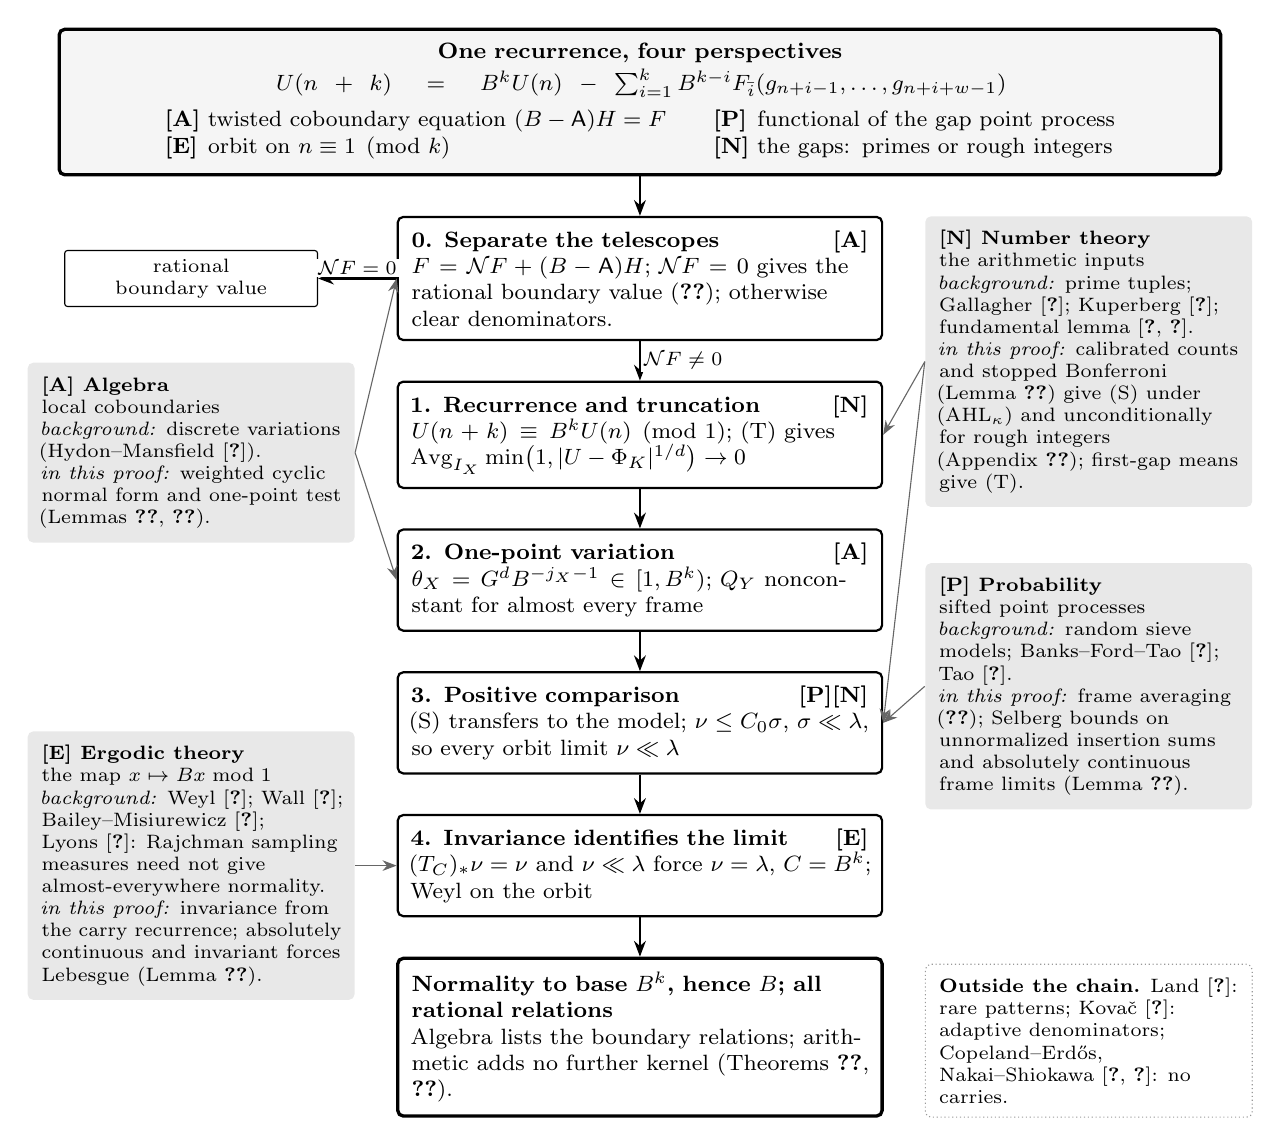
\begin{tikzpicture}[x=1cm,y=1cm,font=\footnotesize,
  head/.style={draw,very thick,rounded corners=2pt,align=center,inner sep=5pt,text width=144mm,fill=black!4},
  stp/.style={draw,thick,rounded corners=2pt,align=left,inner sep=5pt,text width=58mm},
  res/.style={draw,very thick,rounded corners=2pt,align=left,inner sep=5pt,text width=58mm},
  strm/.style={fill=black!9,rounded corners=2pt,align=flush left,inner sep=5pt,text width=38mm,font=\scriptsize},
  arr/.style={-{Stealth[length=2mm]},thick},
  feed/.style={-{Stealth[length=1.8mm]},black!60},
  lab/.style={font=\scriptsize,fill=white,inner sep=1pt}]
 % ---- header ----
 \node[head] (H) at (7.8,0)
   {\textbf{One recurrence, four perspectives}\\[2pt]
    $U(n+k)=B^kU(n)-\sum_{i=1}^{k}B^{k-i}F_{\bar i}(g_{n+i-1},\dots,g_{n+i+w-1})$\\[3pt]
    \begin{tabular}{@{}l@{\ }l@{\qquad}l@{\ }l@{}}
    \textbf{[A]} & twisted coboundary equation $(B-\mathsf A)H=F$ &
    \textbf{[P]} & functional of the gap point process\\
    \textbf{[E]} & orbit on $n\equiv1\pmod k$ &
    \textbf{[N]} & the gaps: primes or rough integers
    \end{tabular}};
 % ---- spine ----
 \node[stp,below=5mm of H] (r0)
   {\textbf{0. Separate the telescopes}\hfill\textbf{[A]}\\
    $F=\mathcal N F+(B-\mathsf A)H$; $\mathcal N F=0$ gives the rational
    boundary value \eqref{eq:localboundary}; otherwise clear denominators.};
 \node[stp,below=5mm of r0] (s1)
   {\textbf{1. Recurrence and truncation}\hfill\textbf{[N]}\\
    $U(n+k)\equiv B^kU(n)\pmod1$;\ 
    (T) gives $\Avg_{I_X}\min\bigl(1,|U-\Phi_K|^{1/d}\bigr)\to0$};
 \node[stp,below=5mm of s1] (s2)
   {\textbf{2. One-point variation}\hfill\textbf{[A]}\\
    $\theta_X=G^dB^{-j_X-1}\in[1,B^k)$; $Q_Y$ nonconstant for almost every frame};
 \node[stp,below=5mm of s2] (s3)
   {\textbf{3. Positive comparison}\hfill\textbf{[P][N]}\\
    (S) transfers to the model; $\nu\le C_0\sigma$, $\sigma\ll\lambda$, so every orbit limit $\nu\ll\lambda$};
 \node[stp,below=5mm of s3] (s4)
   {\textbf{4. Invariance identifies the limit}\hfill\textbf{[E]}\\
    $(T_C)_*\nu=\nu$ and $\nu\ll\lambda$ force $\nu=\lambda$, $C=B^k$; Weyl on the orbit};
 \node[res,below=5mm of s4] (r5)
   {\textbf{Normality to base $B^k$, hence $B$; all rational relations}\\
    Algebra lists the boundary relations; arithmetic adds no further kernel
    (Theorems~\ref{thm:prime}, \ref{thm:rough}).};
 \draw[arr] (H.south)--(r0.north);
 \node[draw,rounded corners=1pt,align=center,font=\scriptsize,text width=30mm,inner sep=3pt] (rat) at (2.1,0 |- r0) {rational\\boundary value};
 \draw[arr] (r0.west)--node[lab,above] {$\mathcal N F=0$}(rat.east);
 \draw[arr] (r0.south)--node[lab,right] {$\mathcal N F\ne0$}(s1.north);
 \draw[arr] (s1.south)--(s2.north);
 \draw[arr] (s2.south)--(s3.north);
 \draw[arr] (s3.south)--(s4.north);
 \draw[arr] (s4.south)--(r5.north);
 % ---- streams: left ----
 \node[strm,below=7mm of rat] (A)
   {\textbf{[A] Algebra}\\ local coboundaries\\
    \emph{background:} discrete variations (Hydon--Mansfield~\cite{hydonmansfield}).\\
    \emph{in this proof:} weighted cyclic normal form and one-point test (Lemmas~\ref{lem:localnormalform}, \ref{lem:onepoint}).};
 \node[strm] (E) at (2.1,0 |- s4)
   {\textbf{[E] Ergodic theory}\\ the map $x\mapsto Bx\bmod1$\\
    \emph{background:} Weyl~\cite{weyl}; Wall~\cite{wall}; Bailey--Misiurewicz~\cite{baileymisiurewicz}; Lyons~\cite{lyons1986}: Rajchman sampling measures need not give almost-everywhere normality.\\
    \emph{in this proof:} invariance from the carry recurrence; absolutely continuous and invariant forces Lebesgue (Lemma~\ref{lem:rigidity}).};
 % ---- streams: right ----
 \node[strm,anchor=north] (N) at (13.5,0 |- r0.north)
   {\textbf{[N] Number theory}\\ the arithmetic inputs\\
    \emph{background:} prime tuples; Gallagher~\cite{gallagher}; Kuperberg~\cite{kuperberg}; fundamental lemma~\cite{friedlanderiwaniec,thornerzaman2019}.\\
    \emph{in this proof:} calibrated counts and stopped Bonferroni (Lemma~\ref{lem:stopped}) give (S) under $(\mathrm{AHL}_\kappa)$ and unconditionally for rough integers (Appendix~\ref{app:rough}); first-gap means give (T).};
 \node[strm,below=7mm of N] (P)
   {\textbf{[P] Probability}\\ sifted point processes\\
    \emph{background:} random sieve models; Banks--Ford--Tao~\cite{bft}; Tao~\cite{tao2023}.\\
    \emph{in this proof:} frame averaging \eqref{eq:frameaverage}; Selberg bounds on unnormalized insertion sums and absolutely continuous frame limits (Lemma~\ref{lem:localspacings}).};
 \node[strm,fill=none,draw=black!40,densely dotted,anchor=south] (O) at (13.5,0 |- r5.south)
   {\textbf{Outside the chain.} Land~\cite{land}: rare patterns; Kova\v c~\cite{kovacforum}: adaptive denominators; Copeland--Erd\H os, Nakai--Shiokawa~\cite{copelanderdoes,nakaishiokawa}: no carries.};
 % ---- feeds ----
 \draw[feed] (A.east) -- (r0.west);
 \draw[feed] (A.east) -- (s2.west);
 \draw[feed] (E.east) -- (s4.west);
 \draw[feed] (N.west) -- (s1.east);
 \draw[feed] (N.west) -- (s3.east);
 \draw[feed] (P.west) -- (s3.east);
\end{tikzpicture}
\caption{Connections behind the proof. The letters mark the viewpoints used by each step. The spine
follows Proposition~\ref{prop:localconsumer} after normal-form reduction,
under its hypotheses and degree bound. The shaded blocks distinguish background from its role in this proof;
(S), (T) are the two arithmetic inputs. The orbit reading uses integral
coefficients and $n\equiv1\pmod k$, with $U(1)=\alpha_F$.
Here $\nu$ is an orbit-limit probability measure, $\lambda$ Lebesgue measure,
$T_C(x)=Cx\bmod1$, and $C_0=24k$. The positive-comparison variant
replaces (S) and multiplies $C_0$ by the fixed factor $c$.}
\label{fig:confluence}
\end{figure}

\clearpage

\phantomsection
\addcontentsline{toc}{section}{References}
\begin{thebibliography}{99}
\bibitem{erdos1988}
P.~Erd\H os, \emph{On the irrationality of certain series: problems and
results}, in A.~Baker (ed.), New Advances in Transcendence Theory,
Cambridge University Press (1988), 102--109.
\href{https://doi.org/10.1017/CBO9780511897184.009}{doi:10.1017/CBO9780511897184.009}.

\bibitem{taoforum}
T.~Tao, comment on Erd\H os Problem~251, 7 October 2025, 17:17.
\url{https://www.erdosproblems.com/forum/thread/251}.
The cited comment suggests quantitative local prime-gap statistics;
it is not a verification of the present result.

\bibitem{kovacforum}
V.~Kova\v{c}, telescoping counterexample for variable product denominators,
comment on Erd\H os Problem~251, 15 April 2026.
\url{https://www.erdosproblems.com/forum/thread/251\#post-5416}.

\bibitem{land}
J.~Land, \emph{A conditional proof of the irrationality of
$\sum p_n/2^n$ under a uniform Hardy--Littlewood prime-tuples conjecture},
research draft, 5 September 2026; public repository and later
conditional Lean formalization.
\url{https://github.com/beetree/math_erdos_251}.
Paper snapshot inspected: commit
\texttt{495dbfee3f947af3fd64b0fd723715ea566c2fb0}.

\bibitem{gallagher}
P.~X.~Gallagher, \emph{On the distribution of primes in short intervals},
Mathematika \textbf{23} (1976), 4--9.
\href{https://doi.org/10.1112/S0025579300016442}{doi:10.1112/S0025579300016442}.

\bibitem{hardylittlewood}
G.~H.~Hardy and J.~E.~Littlewood, \emph{Some problems of `Partitio
numerorum'; III: On the expression of a number as a sum of primes},
Acta Math. \textbf{44} (1923), 1--70.
\href{https://doi.org/10.1007/BF02403921}{doi:10.1007/BF02403921}.

\bibitem{kuperberg}
V.~Kuperberg, \emph{Sums of singular series with large sets and the tail
of the distribution of primes}, Q.~J.~Math. \textbf{74} (2023),
no.~4, 1457--1479.
\href{https://doi.org/10.1093/qmath/haad030}{doi:10.1093/qmath/haad030}.
Conjecture and equation numbering here refer to arXiv:2210.09775v2,
15 June 2023, Conjecture~1.3 and equation~(7):
\url{https://arxiv.org/html/2210.09775v2}.

\bibitem{tao2023}
T.~Tao, \emph{The convergence of an alternating series of Erd\H os,
assuming the Hardy--Littlewood prime tuples conjecture},
arXiv:2308.07205v2 (2023).
\url{https://arxiv.org/html/2308.07205v2}.

\bibitem{bft}
W.~Banks, K.~Ford and T.~Tao, \emph{Large prime gaps and probabilistic
models}, Invent. Math. \textbf{233} (2023), 1471--1518.
\href{https://doi.org/10.1007/s00222-023-01199-0}{doi:10.1007/s00222-023-01199-0};
\url{https://arxiv.org/abs/1908.08613}.

\bibitem{copelanderdoes}
A.~H.~Copeland and P.~Erd\H os, \emph{Note on normal numbers},
Bull. Amer. Math. Soc. \textbf{52} (1946), 857--860.
\href{https://doi.org/10.1090/S0002-9904-1946-08657-7}{doi:10.1090/S0002-9904-1946-08657-7}.

\bibitem{nakaishiokawa}
Y.~Nakai and I.~Shiokawa, \emph{Normality of numbers generated by the values
of polynomials at primes}, Acta Arith. \textbf{81} (1997), 345--356.
\href{https://doi.org/10.4064/aa-81-4-345-356}{doi:10.4064/aa-81-4-345-356}.

\bibitem{madritsch2014}
M.~G.~Madritsch, \emph{Construction of normal numbers via
pseudo-polynomial prime sequences}, Acta Arith. \textbf{166} (2014), 81--99.
\href{https://doi.org/10.4064/aa166-1-7}{doi:10.4064/aa166-1-7}.

\bibitem{baileycrandall}
D.~H.~Bailey and R.~E.~Crandall, \emph{Random generators and normal
numbers}, Experimental Mathematics \textbf{11} (2002), 527--546.
\href{https://doi.org/10.1080/10586458.2002.10504704}{doi:10.1080/10586458.2002.10504704}.

\bibitem{lagarias}
J.~C.~Lagarias, \emph{On the normality of arithmetical constants},
Experimental Mathematics \textbf{10} (2001), 355--368.
\url{https://arxiv.org/abs/math/0101055}.

\bibitem{baileymisiurewicz}
D.~H.~Bailey and M.~Misiurewicz, \emph{A strong hot spot theorem},
Proc. Amer. Math. Soc. \textbf{134} (2006), 2495--2501.
\href{https://doi.org/10.1090/S0002-9939-06-08551-0}{doi:10.1090/S0002-9939-06-08551-0}.

\bibitem{lyons1986}
R.~Lyons, \emph{The measure of non-normal sets}, Invent. Math.
\textbf{83} (1986), 605--616.
\href{https://doi.org/10.1007/BF01394426}{doi:10.1007/BF01394426}.

\bibitem{pratt}
K.~Pratt, \emph{The irrationality of a prime factor series under a
prime tuples conjecture}, arXiv:2409.15185 (2024).
\url{https://arxiv.org/abs/2409.15185}.

\bibitem{taoteravainen}
T.~Tao and J.~Ter\"av\"ainen, \emph{Quantitative correlations and some
problems on prime factors of consecutive integers},
arXiv:2512.01739 (2025).
\url{https://arxiv.org/abs/2512.01739}.

\bibitem{thornerzaman2019}
J.~Thorner and A.~Zaman, \emph{A unified and improved Chebotarev density
theorem}, Algebra Number Theory \textbf{13} (2019), 1039--1068.
\url{https://doi.org/10.2140/ant.2019.13.1039}.

\bibitem{friedlanderiwaniec}
J.~Friedlander and H.~Iwaniec, \emph{Opera de Cribro},
American Mathematical Society Colloquium Publications \textbf{57},
American Mathematical Society, Providence, RI (2010).
\url{https://www.ams.org/books/coll/057/}.

\bibitem{mertens}
F.~Mertens, \emph{Ein Beitrag zur analytischen Zahlentheorie},
J. reine angew. Math. \textbf{78} (1874), 46--62.
\href{https://doi.org/10.1515/crll.1874.78.46}{doi:10.1515/crll.1874.78.46}.

\bibitem{pnt}
C.-J.~de la Vall\'ee Poussin, \emph{Sur la fonction $\zeta(s)$ de Riemann
et le nombre des nombres premiers inf\'erieurs \`a une limite donn\'ee},
M\'emoires couronn\'es et autres m\'emoires, Acad\'emie royale de Belgique,
\textbf{59} (1899), 1--74.
\href{https://doi.org/10.3406/marb.1899.2449}{doi:10.3406/marb.1899.2449}.

\bibitem{montgomeryvaughan}
H.~L.~Montgomery and R.~C.~Vaughan,
\emph{Multiplicative Number Theory I: Classical Theory},
Cambridge University Press (2006).
\href{https://doi.org/10.1017/CBO9780511618314}{doi:10.1017/CBO9780511618314}.

\bibitem{taosieve2015}
T.~Tao, \emph{254A, Notes 4: Some sieve theory}, 21 January 2015,
Theorem~32 and Exercise~34.
\href{https://terrytao.wordpress.com/2015/01/21/254a-notes-4-some-sieve-theory/}{Online lecture notes}.

\bibitem{wall}
D.~D.~Wall, \emph{Normal numbers}, Ph.D. thesis,
University of California, Berkeley (1949).

\bibitem{hydonmansfield}
P.~E.~Hydon and E.~L.~Mansfield, \emph{A variational complex for
difference equations}, Found. Comput. Math. \textbf{4} (2004), 187--217.
\href{https://doi.org/10.1007/s10208-002-0071-9}{doi:10.1007/s10208-002-0071-9}.

\bibitem{weyl}
H.~Weyl, \emph{\"Uber die Gleichverteilung von Zahlen mod.\ Eins},
Math. Ann. \textbf{77} (1916), 313--352.
\href{https://doi.org/10.1007/BF01475864}{doi:10.1007/BF01475864}.

\bibitem{bergelsondownarowicz}
V.~Bergelson and T.~Downarowicz, \emph{On preservation of normality
and determinism under arithmetic operations}, arXiv:2506.12929v1 (2025),
Proposition~4.25 and Remark~4.28.
\url{https://arxiv.org/html/2506.12929v1}.
\end{thebibliography}
\end{document}
